\documentclass[12pt]{article}
\usepackage{class_notes}

\begin{document}
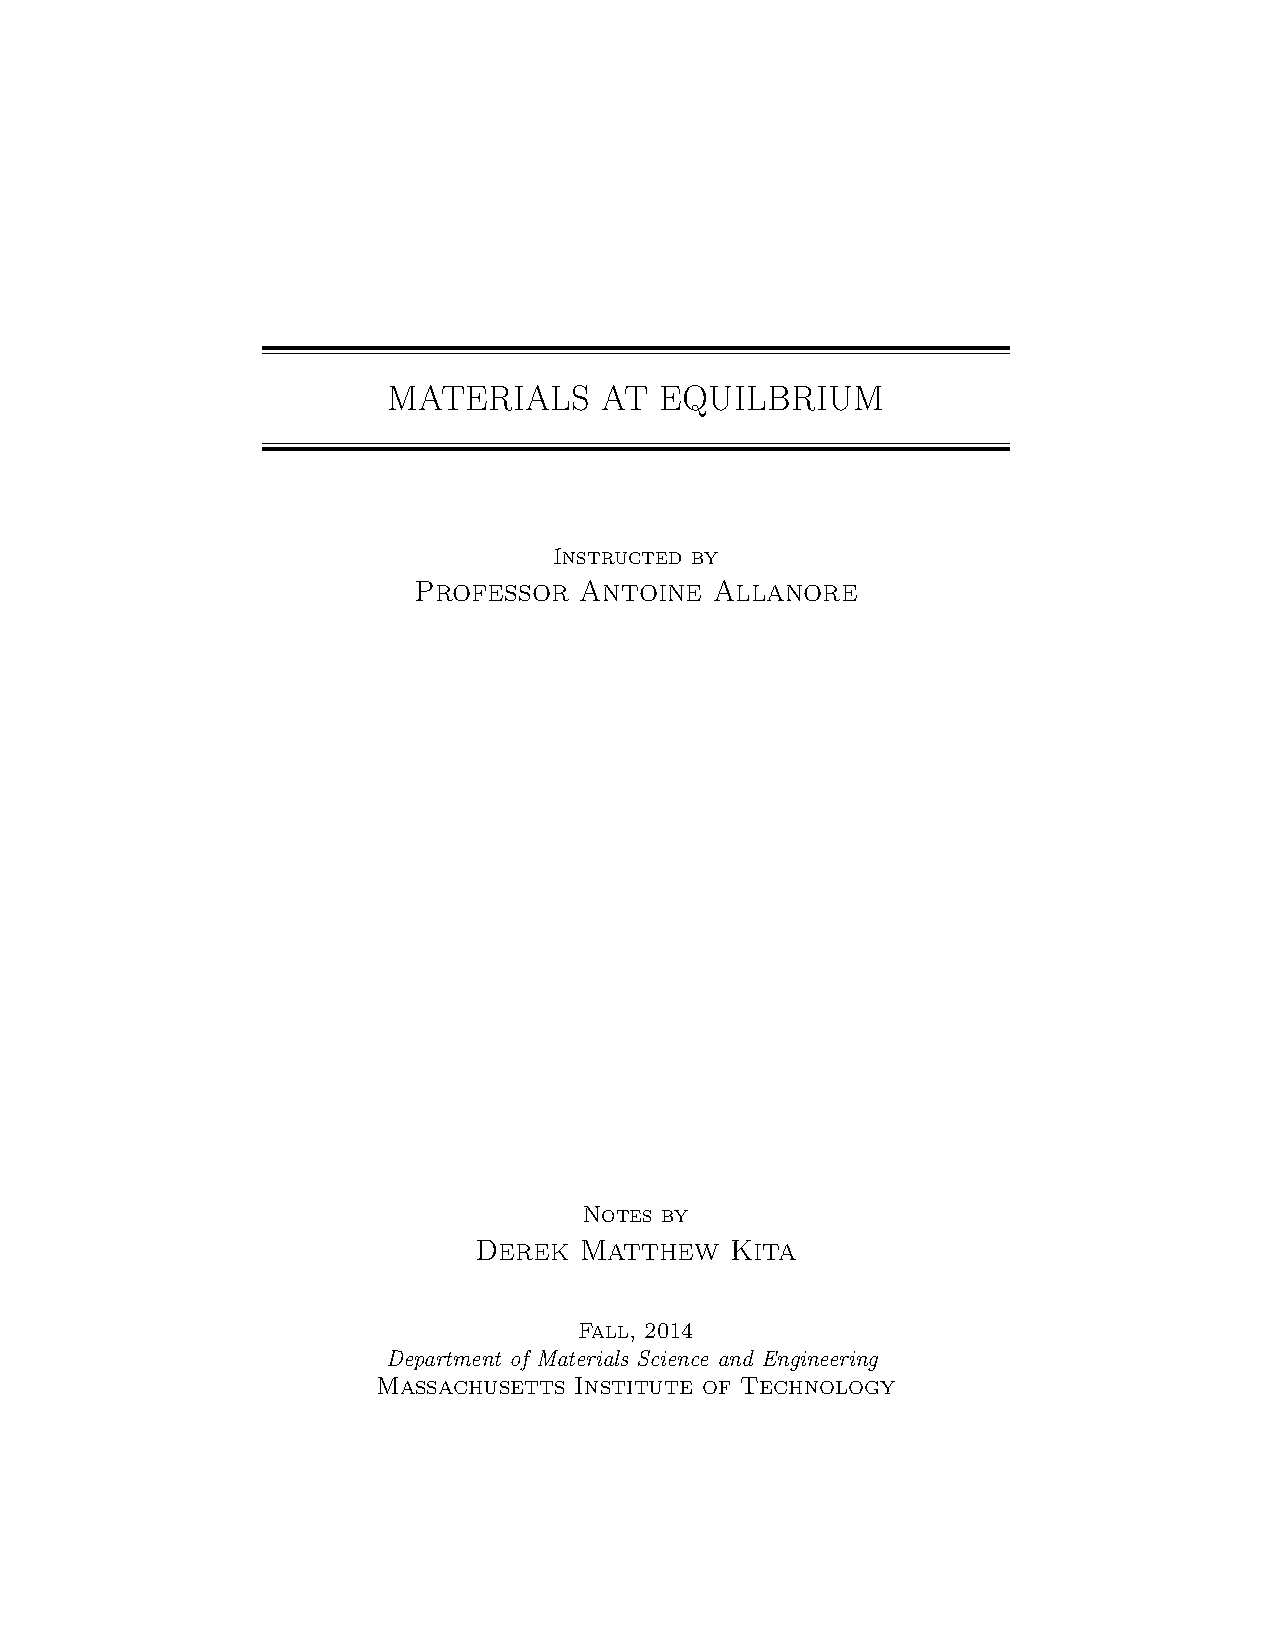
\includepdf[pages=-]{titlepage.pdf}
%%%%%%%%%%%%%%%%%%%%%%%%%%%%%%%%%%%%%%%%%%%%%%%%%%%%%%
\section{Lecture 1: Introduction and Preliminaries}
Welcome to 3.20, Materials at Equilibrium.  This course is designed to provide all incoming students with a grounding in equilibrium thermodynamics.  The material in this course is broadly applicable to all field of materials science and engineering and will serve you well throughout your research as a graduate student.  For information related to the course, including lecture content, problem sets, exams, staff policies, and grading please refer to your course syllabus found on Stellar, or contact the professor directly at \texttt{allanore@mit.edu}.

\subsection{Definitions}
To begin our journey, we will define some frequently used terms for convenience.

\begin{enumerate}
\item \un{System}: Any collection of matter that can be uniquely identified and on which you can define macroscopic averages (a system is not necessarily homogeneous)
\item \un{Environment}: The complement of a system. Together, the system being studied and it's environment make up the universe. 
\eqs
\text{[environment]} = \text{[universe]} - \text{[system]}
\eqe
\item \un{Extensive Variables}: Variables that scale with the system size (i.e. volume, mass, number of particles, $n_{e^-}$, etc.).  If we bring two containers together, the volume is a sum of the individual volumes:
\begin{equation}
V = V_1 + V_2
\end{equation}
\item \un{Intensive Variables}: Variables that are independent of the system size. Intensive variables do \emph{not} scale with system size (i.e. pressure, temperature, E-field, etc.).  For example, the sum of two system's pressures is not equal to the pressure of the sum of both systems:
\eqs
P \neq P_1 + P_2
\eqe
\item \un{State Variables}: The variables required to fully characterize a system (T, P, n, ...).  These are \emph{not} equal to the \bold{state} of a system. However, at equiliibrium, there is a one-to-one mapping between the macroscopic state of the system and the full set of state variables; the state variables fully define the macroscopic equilibrium state.
\item \un{Boundaries}: Conditions that are defined for a system.  These strongly depend on the system of interest. Boundaries can have properties such as: permeable (open to mass flow, changing $n$), impermeable (closed to mass flow), adiabatic (closed to heat flow), diathermal (open to heat flow), rigid (constant volume), deformable, etc. The nature of the boundary defines how the system's state variables can change as it is subjected to different processes. For example, while a system with a rigid boundary is subject to possessing a constant volume during arbitrary processes, a system with a deformable boundary will, for sufficicently slow processes, have the same pressure as its surroundings.
\end{enumerate}

In thermodynamics, we will look at the transfer of energy and other extensive variables at the borders of systems as they undergo processes. Note that this approach treats the system as a black box; we have no idea what is going on microscopically inside the system. We will derive laws regarding the conservation and creation of the extensive variables. Using these laws of conservation, we will be able to define exactly how the macroscopic state of the system changes by only keeping track of what goes on at the boundaries of the system. We will then develop constitutive equations which relate changes in the thermodynamic state variables to one another during arbitrary processes. Integration of these constitutive equations is a powerful and general way to calculate changes in system processes during arbitrary processes. Last, we will use these constitutive relationships to look at a special set of processes; phase transitions, and derive laws for how the conditions under which these phase transitions should occur have to change as the boundary conditions on the system change.

\subsection{Energy and Forces}
What ``forms'' of energy do we have?
\begin{itemize}
\item \un{Potential energy:} Gravitational, electrostatic, etc.
\item \un{Kinetic energy:} Translation, rotations, etc.  
\end{itemize}
This energy can be manifest inside and outside the system.  Other examples of energies are thermal energy (from heat), electromagnetic energy, and chemical energy.
%\begin{equation}
%\Delta E = \Delta E_{ke} + \Delta E_{pe} + \Delta U
%\end{equation}
%where $\Delta U$ is the internal energy.  
For 3.20, we will assume that changes in the total energy $E$ of our system are equal to changes in thr internal energy $U$ of the system.
\begin{equation}
\Delta E = \Delta U
\end{equation}
This is tantamount to neglecting changes in the translational energy of the system as a whole. We assume that $U$ exists, that $U$ is a function of only the extensive thermodynamic variables ($U$ is a \un{state variable}), and that all types of energy exchange that can change the internal state of the system can be represented as work terms represent changes in $U$. We discuss this final assumption next.

%I am not sure 'assumption' is right for some of these; they are not all assumptions... some are implied by others... I think it is fine for teach purposes.

%%%%%%%%%%%%%%%%%%%%%%%%%%%%%%%%%%%%%%%%%%%%%%%%%%%%%%
\section{Lecture 2: Heat and Work}
Let's look at one form of energy transfer: \un{work}. A differential amount of work is equal to the force dotted with the displacement:
\eqs
\delta W = \vec{F} \cdot d\vec{r}
\eqe
The formalism for work is $\delta W_i = y_i dx_i$, where $y_i$ is the force (intensive) and $dx_i$ is the response (extensive). Combined, $(y_i, x_i)$ is a \bold{conjugate pair}.
\subsection{Two examples of work}
\bold{Example 1: Deformation of a material}: The work resulting from a change in strain energy is 
\eqs
\delta W = V \bar{\bar{\sigma}} \cdot d\bar{\bar{\epsilon}}
\eqe 
where the double overbars indicate that $\sigma, \epsilon$ are tensors.  To check the validity of this statement, we note that the stress $\sigma$ has units of [Pa]=[N/$\text{m}^2$], the strain $\epsilon$ is dimensionless, and volume element results in a quantity of [N$\cdot$ m] = [Joules]. We note that the shear stresses in this example are denoted by off-diagonals of $\sigma$ ($\sigma_{12}, \sigma_{13}, \sigma_{23}$).  If we consider only hydrostatic pressure, we will have $\sigma_{11}=\sigma_{22}=\sigma_{33}=-P$.
\eqs
\delta W_\text{pressure} &= V \cdot (-P) d(\epsilon_{11} + \epsilon_{22}+\epsilon_{33})\\
&= -P V (d\epsilon_{11}+d\epsilon_{22}+d\epsilon_{33})
\eqe
We note that the strain is defined as $\epsilon_{11} \equiv \Delta l_1 / l_1^{\text{initial}}$, and $l_1 l_2 l_3 = V$, so we can substitute $V (d\epsilon_{11}+d\epsilon_{22}+d\epsilon_{33}) = dV$:
\begin{equation}
\delta W_\text{pressure} = -P dV
\end{equation}
To solve these, we need an equation of state $P(V)$ or $\sigma(\epsilon)$.  We also have
\begin{equation}
\frac{\partial \epsilon_{ij}}{\partial \sigma_{kl}} = c_{ijkl}
\end{equation}
where $c_{ijkl}$ is the generalized elastic compliance.  If our material is \un{isotropic}, then we will see that $\frac{\partial V}{\partial P}|_T = V \cdot \beta_T$ where $\beta_T$ is the isothermal compressibility - a property of the material that describes volume changes at constant temperature. Hence, using this constitutive relation, $\beta_T(P,T)$, we can define the work done upon the system. \\

\bold{Example 2: Electrical work on an isotropic dielectric medium}: The voltage between two sides of a dielectric is given by the internal electric field and the length as $V = \mathcal{E} \cdot l$.  The energy stored in this capacitor is a product of the voltage and the charge.  If the charge, $q$, changes, we can produce a work term:
\eqs
\delta W = V dq
\eqe
Also, $q=D \cdot A$ where $D$, the electric displacement, is equal to $\varepsilon_0 \mathcal{E} + \frac{\mathcal{P}}{A\cdot l}$.  $\mathcal{P}$ is the total polarization and it is normalized by the volume, $A\cdot l$. We can do some algebra to arrive at a new expression for this work term:
\eqs
\delta W &= \mathcal{E} l  \cdot d(A (\varepsilon_0 \mathcal{E} + \frac{\mathcal{P}}{lA}))\\
&= \mathcal{E}lA \cdot d(\varepsilon_0 \mathcal{E} + \frac{\mathcal{P}}{lA})\\
&= V \varepsilon_0 \mathcal{E} d\mathcal{E} + \mathcal{E} d\mathcal{P}
\eqe

Note how the $\delta W$ nicely seperates into a response that is independent of the system and one that is determined by the material properties of the system. Some energy, $V \varepsilon_0 \mathcal{E} d\mathcal{E}$, is stored even when an electric field is applied to a vacuum. We are not interested in this energy. $\mathcal{E} d\mathcal{P}$, on the other hand, is system-dependent. This is the work term appropriate to the application of an elecric field to a system. You will notice some commonalities between the mechanical work terms discussed previously and the electrical work term: both products result in units of energy, and both can be written as the product of a generalized force (an intensive thermodynamic variable, $P,\mathcal{E}$), and a generalized displacement (an extensive thermodynamic variable, $dV,d\mathcal{P}$). These traits are commmon to all work terms which appear in the internal energy. This implies that changes in the internal energy can be written as a sum over orthogonal work terms:
\eqs
dU = \sum_i y_i dx_i
\eqe
where each $y_i$ represents a generalized force, and each $x_i$ represents a generalized displacement.

We will now discuss how we derive the form of this summation of orthogonal work terms. You might have noticed that we were careful to define the compressibility of a system, $\beta$, over a specific path. Specifically, we defined a compressibility wherein the system was held at constant temperature, $\beta_T$. This is because the compressibility is a function of the boundary conditions under which the compression takes place. \footnote{For example, it takes more energy to compress a gas if you don't let heat flow out of the gas during the compression; the adiabatic compressibility is larger than the isothermal compressiblity.} This concept can be generalized to all work terms: \emph{the work done in changing an extensive variable is a function of the path along which the work takes place}. Put simply, the change in internal energy due to the work terms are \un{path dependent}. In thermodynamics, we make a distinction between path-dependent and path-independent intergrals via exact differentials and inexact differentials. 
\begin{itemize}
\item \un{exact differentials}: The integral of an exact differential path independent; it is only a function of the endpoints.
\item \un{exact differentials}: The integral of an inexact differential is path dependent; the integral depends both on the endpoints and the path to get to these two endpoints.
\end{itemize}
This is illustratted below with two examples.
%%%%%%Next, we can relate this quantity to the characteristic potential energy function of our system.  We know that $\Delta U = U^\text{final} - U^\text{initial}$, and $\delta W = y_i dx_i = F d\vec{r}$.  The force from a potential energy function $\phi$ is $\vec{F}(\vec{r}) = -\vec{\nabla}\phi(\vec{r})$.  Therefore, we have
%%%%%%\begin{align*}
%%%%%%F_x &= -\frac{\partial \phi}{\partial x}|_y \\
%%%%%%F_y &= -\frac{\partial \phi}{\partial y}|_x
%%%%%%\end{align*}
%%%%%%$\vec{F}d\vec{r}$ is an exact differential.  It's integral is path independent.  $\oint \vec{F} \cdot d\vec{r} = 0$.  Also, $\vec{F}$ is a conservative force.  It is like the ``vehicle'' that converts gravitational energy, $E_g$ to electricity.
%%%%%%\begin{align*}
%%%%%%\int_{r_1}^{r_2} \vec{F} d\vec{r} &= \int - \vec{\nabla} \phi(\vec{r})d\vec{r}\\
%%%%%%&= [\phi(\vec{r_2}) - \phi(\vec{r_1})]
%%%%%%\end{align*}

\subsection{Practice with Differentials}
\bold{Case 1, Exact Differentials:}
Consider heights as a function of position, $h(x,y)$.  We will travel from some height $h_1 \rightarrow h_2$.  Anytime we move downwards, we will simply gain kinetic energy.  Anytime we move up a hill, we will first use any kinetic energy we have and then use some stored energy (say, from a battery).  Once we have reached $h_2$, we will give all our kinetic energy to the environment (say from some thermal energy dissipation, like brakes) and we will allow the environment to replenish the energy in our batteries.  The change in potential energy between the two heights is $\Delta E_\text{field}$ and the energy of the environment, i.e. the work required to move us to this new spot, is $\Delta E_\text{system}$.  From conservation of energy,
\eqs
\Delta E_\text{system} + \Delta E_\text{field} = 0
\eqe
Therefore, we can calculate the work required to move us to the new spot via integration of the differential of the gravitational energy with respect to the position (the gravitational force field):
\eqs
\Delta E_\text{field} = dW &= \int \vec{F} \cdot d\vec{r}\\
& = -\int \nabla E_\text{field} \cdot dr\\
& = - mg(h_2 - h_1)
\eqe
Ultimately, the energy change (or work required to move us) from $h_1 \rightarrow h_2$ is independent of the path taken.  Hence, $\vec{F}$ is an exact differential. Mathematicians would say that gravitational force fields are conservative vector fields. This is an equivalence; exact differentials define conservative vector fields.

\bold{Case 2, Inexact Differentials:}  Consider now a system where the force $\vec{F}$ is non-conservative.  The work terms associated with moving through this kind of a vector field are then inexact differentials. \un{dissipative forces} tend to make the force vector-field non-conservative, resulting in path dependence. For example, moving in a gravitational field with a constant friction term would result in:
\begin{align*}
\vec{F} &= -\vec{\nabla}\vec{E} - f_\text{friction} | \vec{e_v}|\\
\int \vec{F}\delta\vec{r} &= -mg\Delta h- f L_\text{path}
\end{align*} 

 In thermodynamics, you can get an inexact differential for two reasons. As described above, dissipation leads to inexact differentials. A second, related way, is simply not taking into account all of the forces during your integration. Such an incomplete description will result in path-dependent integrals, even if the underlieing vector field is conservative. For example, if we are moving in three dimensions and do not describe the force in the $y$-direction, $F_y'$, then we would (incorrectly) describe the work when moving in three dimensions as:
\begin{align*}
\delta W_\text{incomplete} = \delta W_x + \delta W_z = F_x \dot dx + F_z \dot dz 
\end{align*}
Consider two different paths in a conservative 3D vector field.  The integrated amount of work done due to the x- and z- forces may be different between the two paths, even though the total work is the same. This results in a path dependence in the energy acquired while moving.  For path \#1 we might have $\int \delta W_x + \delta W_z = \int F_x dx F_z dz = 0$ whereas for path \#2 we could very well have $W_x = \int F_x dx \neq 0$.  This is analogous to describing the changes in internal energy of a system through only work terms; we are missing an entire component of the internal energy change, the change to due to \un{heat} flow into a system.



\subsection{Heat}
Heat is energy transferred between two bodies not due to work or mass transfer.
\footnote{Historically, people used to think heat was transferred between bodies via the flow of an invisibile substance, \textit{phlogiston}. Hot bodies contained more of this self-repelling fluid than cold bodies. Two heros of science helped disprove this crazy theory. First, Antoine Lavoisier showed that metals gained mass when they oxidized, even though they were supposed to lose phlogiston, so phlogiston would need to have negative mass. This lead to phlogiston theory being replaced by caloric theory, in which calor, another invisble liquid, flowed from hot to cold bodies. All caloric theories assumed that calor was conserved. Sir Benjamin Thompson (AKA Lord Rumford) disproved this theory by showing that repeatedly boring a cannon could repeatedly produce heat, showing that heat was not a conserved quantity, but rather, could be generated. This lead to Rudolf Clausius proposing that it is not heat which is conserved, but rather energy. This was the birth of modern thermodynamics.}  The variable we will use to denote heat is $Q$.  A system surrounded by an adiabatic boundary does not transfer heat across its boundaries, and so we say the heat exhanged between the system and the surroundings is 0; $\delta Q = 0$.  The \un{first postulate of thermodynamics} is
\begin{equation}\boxed{
dU = \delta W + \delta Q
}\end{equation}
The value of $U$ is path independent via the conservation of energy. As such, $U$ is a function of solely the system's state. Appropriately, functions which are completely defined by the thermodynamic state of the system are called \un{state functions}; their differentials must thus be exact differentials. On the contrary, $W$ and $Q$ are \un{path dependent}; transfer of energy can be accomplished in a multitude of ways.  This is why we write both changes in heat and work with the inexact differential symbol, $\delta$, but the sum of the two as $dU$.

\bold{Example:} Consider a simple system with all variables fixed except for the volume, like a piston.  It then evolves ``slowly'' through a series of equilibrium states.\footnote{We call such infinitely slow processes, where in the system can be approximated as being in equilibrium the whole time  \un{quasistatic processes}.}  
\eqs
W = -\int P dV
\eqe
Assuming we are dealing with an ideal gas, we have the following equation of state $P = \frac{nRT}{V}$.  Inserting this into the above (and assuming constant temperature), we have an expression for work in terms of the initial and final volumes.
\eqs
W &= -nRT\int \frac{dV}{V}\\
&= nRT \ln\Big(\frac{V_f}{V_i}\Big)
\eqe
It is often useful to think of these changes as paths in a pressure versus volume plot.  Let's consider a path $a$ where both the pressure and volume can change.  We will compress the gas isothermally from a volume $V_1$ to a final volume $V_f = V_1/2$.  Also, we are at room temperature, $T=298K$.
%%%% We should insert the relevant P-V diagram here!
\eqs
W_a &= -nRT\int \frac{dV}{V}\\
&= -nRT \ln(\frac{V_f}{V_i})\\
&= nRT \ln(2)\\
&= 1717 \frac{\text{J}}{\text{mol}}
\eqe
Let's now consider a separate path $b$ that is first isobarically compressed ($dP=0$), and then isochorically warmed ($dV = 0$), such that both the initial and final states are the same as those in $a$.  For the constant volume pressure change, there will be no work done since $dV=0$ and $W=-PdV$.  Therefore all the work will come from the initial constant pressure process, or isobaric compression.
\begin{align*}
W_b &= -P_i \int dV\\
&= \frac{P_i V_i}{2}\\
&= \frac{nRT}{2}\\
&= 1239 \frac{\text{J}}{\text{mol}}
\end{align*}

Clearly, the amount of work done when changing between two states can be different, although the change in internal energy must be the same. Thus, there must have been different amounts of heat transferred along each path as well; both work and heat are path-dependent.

%%%%%%%%%%%%%%%%%%%%%%%%%%%%%%%%%%%%%%%%%%%%%%%%%%%%%
%\section{Lecture - September 8, 2014}
%Last time, we had $dU = \partial Q + \sum y_i dx_i$.  
%\subsection{Today}
%We now want to quantify the first term, or \un{quantify heat exchange}.  We do this by defining a heat capacity in closed system (normalized by $n$) via
%\begin{equation}
%C_\text{path} = \frac{1}{n} \frac{(\partial Q)_\text{path}}{dT}
%\end{equation}
%This is the specific heat capacity.  If we consider a \un{simple system} with state variables $(P,V)$ or $(V,T)$, we can define
%\begin{align*}
%C_p &= \frac{1}{n} \frac{(\partial Q)_p}{dT}\\
%C_v &=  \frac{1}{n} \frac{(\partial Q)_v}{dT}
%\end{align*}
%We can wonder what is larger, $C_p$ or $C_v$.  Look at Figure 1 on sheet.  At constant $V$, $\Delta U = Q$.  At constant $P$, $\Delta U = Q + W = Q - p dV$.  Both $\Delta U$ and $dT$ will be less.\\
%
%(a) \un{gases}: We assume they are ideal gases (non interacting, hard spheres).  We get $\frac{1}{2} R$ per degree of freedom.
%\begin{equation}
%C_v = \frac{3}{3} R
%\end{equation}
%for monoatomic gas.  $R = 8314 \text{J}/\text{mol}/\text{K}$ and $R = N_a \times k_B$.  For a diatomic gas, with two atoms attached by a spring, we have between 6 and 1 degrees of freedom.  We will get $C_v = \frac{5}{2} R$.
%
%\begin{align*}
%C_p &= C_v + R\\
%&= \frac{7}{2} R =  29 \text{J}/\text{mol}/\text{K}
%\end{align*}
%
%(b) \un{solids}: At room temp., for an element, Dulong and Petit (1819) predicted
%\begin{align*}
%C_v &\approx 3 R = 25 \text{J}/\text{mol}/\text{K}\\
%C_p & \approx C_v
%\end{align*}
%For a non metallic salt (i.e. MgO), $C_p \approx 6 R = 50\text{J}/\text{mol}/\text{K}$.  Now we look at the Practical $C_p$ from the handouts sheet.  We can see that at high T carbon reaches the 3 R.  It takes a while to reach this because of the nature of carbon's covalent bonds.  There are points in Fe's diagram at 1550 \degree C because at this point it melts.  Same with Hg, which becomes a gas at low T.  For H\2O at RT we have $C_p = 75 \text{J}/\text{mol}/\text{K}$.
%
%\subsection{We need another energy function}
%Now, we will define a term called the \bold{enthalpy} $H$
%\begin{align*}
%H &= U + PV\\
%dH &= dU + V dP + P dV
%\end{align*}
%and substitute $dU = \partial Q - P dV$
%\begin{align*}
%dH &= \partial Q + V dP\\
%(dH)_p &= \partial Q
%\end{align*}
%and now we have a new function of state that describes the heat change at constant pressure.  With this we can perform \un{calorimetry} which is an indication of the heat exchange at constant P.  We can call this $(dH)_p$ the ``heat'' content.\\
%
%If we write down what $(dH)_p$ is, we get
%\begin{align*}
%(dH)_p &= n C_p (dT)_p\\
%\frac{\partial H}{\partial T}|_p &= C_p\\
%H(T) &= H(T_0) + n C_p \Delta T + \Delta H_{\phi T}
%\end{align*}
%where first term is the reference T from the reference state and $\phi T$ is ``phase transformation''.  By definition, $H=0$ for an element at atmospheric pressure ($P_0 = 101325$ Pa) and temperature ($T_0 = 298$ K).\\
%
%The standard state is the form most stable or common at room T or pressure (i.e. O\2(g), Hg(l), C(graphite)).
%
%On the second sheet of the handout (H\degree(Fe)) we see the standard molar enthalpy with changing T.  The slope of this chart is $\frac{(dH)_p}{dT}$ which is the heat capacity.  Beneath 900\degree C, we have $\alpha$ BCC phase, at $900^0 < T < 1400^0$ we have $\gamma$ FCC, then roughly to 1500\degree we have $\delta$ BCC and above this the liquid phase.
%
%$\Delta H_\text{Fe}^{\alpha \rightarrow \gamma} \approx 1$ kJ/mol and $\Delta H_\text{Fe}^{\gamma \rightarrow \delta} \approx 1$ kJ/mol.
%
%$\Delta H_{\text{ZrO}_2}^{\text{tetra}\rightarrow \text{non}} \approx 6$ kJ/mol.  Richard's rule says that
%\begin{equation}
%\Delta H_\text{fusion} \approx 9 T_\text{fusion}
%\end{equation}
%with T in Kelvin.  In most elements this is around 10 kJ/mol.  The heat of vaporization follows roughly Trouton's rule
%\begin{equation}
%\Delta H_\text{vap} \approx 90 T_\text{vap}
%\end{equation}
%In most elements this is around 100 kJ/mol.  At these phase transformations, we are talking about binding energy, which can be roughly 1 eV/atom.  1 F $\cdot$ 1 eV is roughly 100 kJ/mol.\\
%
%Now, what about the significance of that PdV term?  Perform a phase transformation from phase I $\rightarrow$ phase II.  In a metal, $\rho \approx 10$ cm$^3$ / mol and we assume 10\% $\Delta V$.  P\degree = 101325 Pa and thus $P \Delta V = 10^5 \cdot 10^{-6} = 0.1$.
%%
%%(c) \un{compounds}: At RT and P\degree
%%\begin{equation}
%%2 Fe_{(s)} + \frac{3}{2} + O_{2 (g)} \rightarrow \alpha-Fe_2O_{3 (s)} + (\partial Q)_p
%%\end{equation}
%%with $(\partial Q)_p$ = -1963 kcal/mol.
%%\begin{equation}
%%\Delta_v H = \Delta H^0_{Fe_2O_3} - \Delta H^0_{Fe} - \frac{3}{2} \Delta H^0_{O_2}
%%\end{equation}
%%and
%%\begin{align*}
%%\Delta H^0_{Fe_2O_3} &= -820.5 \text{kJ}/\text{mol}\\
%%\Delta H^0_{CO} &= -110.52 \text{kJ}/\text{mol}\\
%%\Delta H^0_{CO_2} &= -393.51 \cdot \text{kJ}/\text{mol}
%%\end{align*}
%%
%%There are plenty of references to get these values, such as \un{Janaf tables}.  Examples include FactSage \& Thermocalc and they provide $H^0$, $G^0$, $C_p^0$, etc.
%%
%%\begin{align*}
%%C_{(s)} + O_{2 (g)} &\rightleftharpoons CO_{2 (g)}\\
%%\Delta_r H^0 &= -393.52 \text{kJ}/\text{mol}\\
%%C_{(s)} + \frac{1}{2} O_{2 (g)} &\rightleftharpoons CO_{(g)}\\
%%\Delta_r H^0 &= -110.52 \text{kJ}/\text{mol}\\
%%C_{(s)} + CO_{2 (g)} &\rightleftharpoons 2 CO_{(g)}\\
%%\Delta_r H^0 &= +180 \text{kJ}/\text{mol}\\
%%\end{align*}
%%
%%The $\Delta H$ only tells you how much heat is exchanged, it doesn't tell you which reaction is \emph{going to happen}.  Be careful with the idea of ``heat'' content.  Doesn't mean we're going to harvest this energy as heat.  The first law is also silent about the directions of change $\rightleftharpoons$.  The first of the three reactions above is exothermic and the last is endothermic.
%%
%%%%%%%%%%%%%%%%%%%%%%%%%%%%%%%%%%%%%%%%%%%%%%%%%%%%%%%%
%\section{Lecture - September 9, 2014}
%In previous lectures we worked with the first law with both the heat and work terms.  In continuation, imagine we have a lightbulb.  We can model the work as
%\begin{align*}
%W_\text{electric} = \partial Q + E_{\hbar v}
%\end{align*}
%If we have two compartments that are connected, one at $T_1$ and another at $T_2$ with $T_1 > T_2$ and $Q_1 < 0$ \& $Q_2 > 0$.
%
%\subsection{Different types of processes}
%\bold{With ideal gas}:  This is nice because we can probe the internal energy U(T) by only looking at the temperature (the only ``state'' variable).  If we have a bike tube initially at RT with $P=4.4$atm (50 psi) and $T=298K$.  Now, we release the pressure from the bike tire and let air out.  What will happen to the temperature of the air right outside the nozzle.\\
%
%First, we have adiabatic expansion (not enough time for system to exchange heat).
%\begin{align*}
%dU_\text{gas} &= \partial Q + \partial W\\
%&= -P dV\\
%&= n C_V dT = -P dV
%\end{align*}
%Note that
%\begin{align*}
%V &= nR\frac{T}{P}\\
%dV &= \frac{n R}{P} dT - nRT \frac{dP}{P^2}
%\end{align*}
%
%So that
%\begin{align*}
%nC_V dT &= -nRdT + RT \frac{dP}{P}\\
%(\frac{T_2}{T_1})^{C_P/ R} &= \frac{P_2}{P_1}\\
%T_2 &= T_1 (\frac{P_1}{P_2})^{R/C_P}
%\end{align*}
%
%And plugging in, we have $T_2 = 206$K = -67\degree C.  Why didn't we actually reach this temperature?  Well, the gas flowed through a nozzle instead of being simple allowed to expand.\\
%
%\bold{What is happening through the valve?}  \un{Joule-Thompson expansion} our system is the valve.  
%\begin{equation}
%dU_\text{valve} = U_\text{in} \partial n - U_\text{out} \partial n + \partial Q
%\end{equation}
%The gas enters with $P_\text{in}$ and a specific volume $V_\text{in}$ then leaves with $P_\text{out}$ and $V_\text{out}$.  Even though this is a constant volume system, the fact that we are flowing matter means we will have a work term.
%\begin{equation}
%dU_\text{valve} = \partial n (P_\text{in} V_\text{in} - P_\text{out} V_\text{out})
%\end{equation}
%The valve is an \un{open system} (can exchange particles with environment), and since it is in the steady state we have $dU_\text{valve} = 0$.
%
%\begin{align*}
%(U_\text{in} - U_\text{out}) &= (P_\text{in} V_\text{in} - P_\text{out} V_\text{out})\\
%n C_V dT &= nR(\Delta T)\\
%\end{align*}
%There is a problem with the above.  It says either $C_V = R$, or $\boxed{\Delta T=0}$.
%
%We have a Joule-Thompson, irreversible process.  It is dissipative and not at equilibrium with environment.
%We need to know what kinds of processes are involved to appropriately treat our system.  Please refer to \bold{Callen pg. 95}.
%
%\begin{enumerate}[(I)]
%\item Continuous and at equilibrium with environment (reversible). See Figure 2.
%\item Continuous but not necessarily at equilibrium with environment.  This is considered \un{quasi-static}.  Can be both reversible and irreversible.  See Figure 3.
%\item Discontinuous and not in equilibrium.  We can not do equilibrium thermodynamics for this.  (i.e. an explosion with H\2 + O\2 will proceed so fast we can not tell what is happening to get us to the final stage.  See Figure 4.
%\end{enumerate}
%
%\subsection{Quasistatic Piston}
%See Figure 5.  For our path,
%\begin{equation}
%\sum_{i=1}^2 \frac{\partial Q_i}{T} = \text{constant}
%\end{equation}
%Only depends on 1 (initial state) and 2 (final state).  The above is also our state function.\\
%
%Let's assume that $dS = \frac{\partial Q}{T}$.\\
%\bold{Process 1}: Let's take a reservoir that is adiabatically isolated with $T_1$.  Let's transfer $\partial Q$ to the reservoir.  The resulting temperature will then be $T_2$.\\
%\bold{Process 2:} Now we have a propeller going into our reservoir with adiabatic walls and $T_1$.  Here, we have $dS_1 = dS_2 \neq \frac{\partial Q}{T}$.\\
%
%Second Law of Thermodynamics:  There exists a state function (property S) for which holds (closed system)
%\begin{equation}
%dS_\text{system} \geq \frac{\partial Q}{T}
%\end{equation}
%it fixes the direction of change.  Forward ($1\rightarrow 2$) if $dS_f \geq \frac{\partial Q_f}{T}$ or backward ($2\rightarrow 1$) if $dS_b \geq \frac{\partial Q_b}{T}$.\\
%
%If a process is \un{reversible} (quasi-static), then we have $dS = \frac{\partial Q}{T}$.  If it is \un{irreversible}, $dS > \frac{\partial Q}{T}$ (or $dS_\text{rev} + \xi$ where $\xi >0$).  The first law said that $U$ exists and
%\begin{equation}
%dU = \partial Q + \sum y_i dx_i
%\end{equation}
%while the second law says $S$ exists and for a closed system
%\begin{equation}
%dS \geq \frac{\partial Q}{T}
%\end{equation}
%
%Back to the example of two compartments that are connected (one at $T_1$ and the other at $T_2$), see Figure 6, we get
%\begin{align*}
%\partial Q_1 &= -\partial Q_2\\
%dS_\text{system} &= dS_1 + dS_2\\
%dS_\text{system} &= \frac{\partial Q_1}{T_1} + \frac{\partial Q_2}{T_2}\\
%&= \frac{\partial Q_1}{T_1} - \frac{\partial Q_1}{T_2}\\
%&= \partial Q_1 (\frac{1}{T_1} - \frac{1}{T_2})\\
%&= \partial Q_1 (\frac{T_2 - T_1}{T_1 T_2}) \geq 0\\
%\end{align*}
%If $T_2 > T_1$, $\partial Q_1 > 0$.  Or if $T_2 < T_1$, then $\partial Q_1 < 0$.  Heat flows from ``hot'' to ``cold''.
%
%%%%%%%%%%%%%%%%%%%%%%%%%%%%%%%%%%%%%%%%%%%%%%%%%%%%%%%
%\section{Lecture - September 10, 2014}
%As a reminder, the 1st law stated that $U$ is a state function where
%\beq
%dU = \partial Q + \sum y_i dx_i
%\ceq
%The 2nd law states that $S$ is also a state function, and for a \emph{closed system}
%\beq dS \geq \frac{\partial Q}{T} \ceq
%If quasi static and reversible then it is equal.  The change in the entropy for the entire system must increase ($dS_\text{system} \geq 0$).
%Key comments
%\begin{enumerate}[(I)]
%\item $S$ is not a conserved quantity.  Imagine the case where we stir an isolated bucket (with a propeller).
%\item $S$ of an adiabatic system increases.  This is because the $\partial Q$ term is zero, so $dS \geq 0$.
%\item $S$ \emph{can} decrease.  An example is allowing liquid iron to cool and form a solid phase.  In this case the entropy decreases.  The entropy of the environment, however, increases by an amount much greater than the decrease of iron entropy.  Thus, $dS_\text{universe}$ is positive.
%\end{enumerate}
%\subsection{Consequences of the 2nd law:}
%\begin{enumerate}[(I)]
%\item The work done for a reversible process is less than or equal to the work done for an irreversible process
%\beq \partial W_\text{reversible} \leq \partial W_\text{irreversible} \ceq
%For a reversible path, \beq dU_\text{reversible} = \partial Q_\text{reversible} + \partial W_\text{reversible} \ceq
%and the second law allows us to replace $\partial Q_\text{reversible}$ by $TdS$.  For an irreversible path,
%\beq dU_\text{irreversible} = dU_\text{reversible} = \partial Q_\text{irreversible} + \partial W_\text{irreversible} \ceq
%Since $\partial Q_\text{irreversible} < T dS$ for an irreversible process, we have
%\beq T dS + \partial W_\text{reversible} > T dS + \partial W_\text{irreversible}
%\ceq
%and 
%\beq \boxed{\partial W_\text{reversible} > \partial W_\text{irreversible}}
%\ceq
%\item \un{limits to work conversion}: For a reversible process, we will get the most efficient conversion.
%\begin{align*}
%\Delta U = 0 &= Q + W\\
%\Delta S = \oint \frac{\partial Q}{T}& = 0\\
%&= \frac{Q_H}{T_H}
%\end{align*}
%\begin{align*}
%\oint \frac{\partial Q}{T} &= 0\\
%\Delta S &= \frac{Q_H}{T_H} + \frac{Q_L}{T_L}\\
%&= 0\\
%Q_H &= \frac{-T_L}{T_H} Q_L
%\end{align*}
%\begin{align*}
%Q &= -W\\
%Q_H + Q_L &= -W\\
%Q_H - Q_H \frac{T_L}{T_H} = -W\\
%Q_H (1 - \frac{T_L}{T_H}) = -W\\
%\end{align*}
%This gives us the Carnot efficiency $\eta = \frac{-W}{Q_H}$ and \beq \eta = 1 - \frac{T_L}{T_H} \ceq  Now, plugging in numbers, with $T_H = 100^0$ C = 373 K and $T_L$ = 25\degree C = 298 K, $\eta \approx 20$\%. and if $T_H$ = 550\degree C, $\eta \approx 63$\%.
%
%We use work to flow \un{heat}.  With $Q_H$ leaving we have a \un{heat pump} and $Q_L$ coming in we have a refrigerator.
%\beq \eta_\text{heat pump} = \frac{-Q_H}{W} = \frac{T_H}{T_H - T_L} \ceq
%With $T_H = 25$C and $T_C = 0$C, $\eta = 11\phi$ ($\phi$ is the ``coefficient of performance''?).
%\end{enumerate}
%
%\un{Practically}, we use a fluid for heat transfer.  We add heat $Q_H$ to water that turns into steam and runs a turbine generating work $W$.  We take some heat $Q_L$ away from this so it can condense and we flow it back to the top.  We can have inefficiencies turning the turbine, condensing the steam back into water, etc.
%
%We will compute the entropy $S$ for materials.  We know the temperature dependence
%\beq C_c = \frac{(\partial Q)_c}{dT} \ceq
%Where the subscript c is for ``constant path''.
%\begin{align*}
%T(dS)_c &= (\partial Q)_c\\
%T(\frac{\partial S}{\partial T})_p &= C_p\\
%T(\frac{\partial S}{\partial T})_v &= C_v\\
%\end{align*}
%Fun fact: thermoelectrics will never be as efficient as steam engines (see Nature Materials Vol 8 Feb 2009 ``An inconvenient truth about thermoelectrics'').
%
%Ultimately, we need a reference state.  How do we come up with a reference entropy $S$?  Nernst got the Nobel prize for it in 1920.
%
%\subsection{The 3rd law}
%\emph{As the temperature approaches zero, the magnitude of the entropy change in any reversible process is zero.}
%We can then fix the entropy of the elements at 0K, in their \un{equilibrium} state, at zero. \beq S_{0\text{K}}^0 = 0 \ceq
%\beq A + B \rightarrow AB \text{  (at 0K})\ceq
%With this process $\Delta S = 0$ (reversible path) and $S_{AB}^\text{0K} = 0$.  Alternatively, it can be said that ``The entropy of a system at 0K is 0''.  This statement, however,is true if we are at \un{equilibrium}.\\
%
%Looking at the Entropy vs. Temperature handout, we see that the phase transformation at $\sim 900$\degree C results in a jump in both entropy and enthalpy.  $S$ is an extensive property and a state function.  For the $\alpha \rightarrow \gamma$ phase transformation
%\beq \Delta S_{\alpha \rightarrow \gamma} = \frac{\Delta H_{\alpha \rightarrow \gamma}}{T_{\phi T}} \ceq
%Say that we go from liquid to vapor, what is $\Delta S_{(l) \rightarrow (v)}$?  T $\approx$ 3000.\\
%
%\un{Trouton's rules}: $\Delta H_\text{vaporization} = 90 \times T_\text{vaporization}$.  With this, $\Delta S_\text{vaporization} \approx 90 \frac{J}{\text{mol} K}$.
%
%\bold{Can we reach 0K?}
%Consider $T_\text{outside}$ = 25\degree C and $T_\text{chamber} \approx  0.1$K.  We need to extract heat and place it in an adiabatic environment.  See Figure 5.1.  We can reduce the temperature by cycling between isothermal compression and isentropic (adiabatic?) expansion, but we can never practically use this method to get to 0K.
%\begin{enumerate}[(I)]
%\item \un{Adiabatic expansion} of an ideal gas.  How much entropy changes?
%\beq T_2/T_1 = \frac{P_1}{P_2}^{R/C_v} \ceq
%Don't do this.  Just look at the \un{adiabatic} part and jump to $dS = 0$
%\item \un{Isothermal} reversible expansion of an ideal gas.  $dS = \frac{\partial Q}{T} = -\frac{\partial Q}{T} = \frac{PdV}{T} = nR \frac{dV}{V}$ (Know this since $U(T)$, with T constant means $\Delta U = 0 = Q + W$)
%\beq \Delta S = nR\ln(\frac{V_2}{V_1}) \ceq
%As volume goes up, entropy will too.
%\item Arbitrary change of an ideal gas.  Since $S$ is a state function, we only need to find the reversible path.  We can break it up:
%\beq dS = dS_\text{isobaric} + dS_\text{isothermal} = C_p \frac{dT}{T} - R\frac{dP}{P} \ceq
%
%\end{enumerate}
%
%%%%%%%%%%%%%%%%%%%%%%%%%%%%%%%%%%%%%%%%%%%%%%%%%%%%%%%
%\section{Lecture - September 12, 2014}
%We can perform a Legendre Transformation to come up with new representations of our system's energy
%\eqs
%dU = TdS + \sum_i y_i dx_i
%\eqe
%Lets consider a simple system.  We can write it in terms of several ``natural functions'' ($U(S,V)$ or $S(U,V)$)
%\eqs
%dU &= T dS - P dV\\
%dS &= \frac{1}{T}dU + \frac{P}{T}dV
%\eqe
%also, we may integrate our function
%\eqs
%U(S,X_i) \rightarrow dU = \frac{\partial U}{\partial S}|_{X_i} dS + \frac{\partial U}{\partial X_j}|_{X_{i\neq j}} dX_j
%\eqe
%and thus we have relations for our equations of state
%\eqs
%T(S,X_i) &= \frac{\partial U}{\partial S}|_{X_i}\\
%y_j(S,X_j) &= \frac{\partial U}{\partial X_j}|_{X_{i\neq j}} 
%\eqe
%If we just have one equation of state ($T(S,V)$), we can get
%\eqs
%U = \int dS T(S,V) + g_1(V)
%\eqe
%similarly if we only have $-P$
%\eqs
%U = -\int dV P(S,V) + g_2(S)
%\eqe
%The number of ways the system can exchange energy is equal to the number of equations of state (EOS).
%\subsection{Mathematical Properties of $U$}
%$U$ is a homogeneous function of first order in \emph{extensive} variables.
%\eqs
%f(\lambda x, \lambda ) = \lambda^r f(x,y)
%\eqe
%taking $r=1$ for $U$,
%\eqs
%f(\lambda x, \lambda y) = \lambda f(x,y)
%\eqe
%lets verify the result:
%\eqs
%\frac{\partial (U(\lambda S, \lambda X))}{\partial \lambda} &= \frac{\partial U}{\partial (\lambda S)} \frac{\partial (\lambda S)}{\partial \lambda} + \frac{\partial U}{\partial (\lambda X)} \frac{\partial (\lambda X)}{\partial \lambda}\\
%&= \frac{\partial U}{\partial (\lambda S)} S + \frac{\partial U}{\partial (\lambda X)}X\\
%&= \frac{\partial U}{\partial S} S + \frac{\partial U}{\partial X} X\\
%&= U(S,X)
%\eqe
%Thus for $\lambda = 1$
%\eqs
%U = TS + yx
%\eqe
%\subsection{An open and isolated system}
%Now we consider the chemical potential $\mu$, the intensive conjugate of $dN$ which is the change in number of particles:
%\eqs
%U &= TS - PV + \sum_i \mu_i N_i\\
%dU &= SdT - VdP + N_i d\mu_i = 0
%\eqe
%where the above is called the ``Gibbs-Duhem equation''
%
%For an isolated system, we have no dV, no dU.  The 1st law says $U, V$ are constant (no energy flow) and the 2nd law says $dS \geq 0$ (i.e. S is maximized over the set of thermodynamic states that are consistent with the extensive variable constraints (boundaries).  The most probable thermodynamic state is then the one with the maximum S.\\
%
%Lets look at thermal equilibrium (Temperature differences) in a system with two containers that allow energy to flow $dU \neq 0$.
%\eqs
%dU_I &= -dU_{II}\\
%dS &= dS_I + dS_{II}\\
%dS &= \frac{dU_I}{T_I} + \frac{dU_{II}}{T_{II}}\\
%dS &= dU_I (\frac{1}{T_I}+\frac{1}{T_{II}})
%\eqe
%Now, if $T_I < T_{II}$ and $dU_I > 0$, then $dS > 0$ and we are \bold{not at equilibrium}.  If $T_I > T_{II}$ and $dU_I < 0$, then $dS > 0$ and we are also \bold{not at equilibrium}.  Equilibrium then occurs when $\frac{1}{T_I}+\frac{1}{T_{II}} = 0$, or $T_I = T_{II}$.
%
%\subsection{Mechanical Equilibrium}
%Consider two compartments of an isolated container separated by an athermal, moveable wall.  The volume of the left side is $V_1$ and the right is $V_2$.
%\eqs
%dU_1 &= -dU_2\\
%dV_1 &= -dV_2\\
%dS &= dU_1 (\frac{1}{T_1}+\frac{1}{T_{2}}) + dV_1 (\frac{P_1}{T_1}+\frac{P_2}{T_{2}})\\
%\eqe
%thus $S$ is maximal for $T_1 = T_2$ and $P_1 = P_2$.
%\subsection*{Chemical Equilibrium}
%Similarly, we can add a $\mu dN$ term to the energy change (or $-\frac{\mu}{T}dN$ in the entropy representation).  We then get an additional term to $dS$ of 
%\eqs
%dS = ... -(\frac{\mu_1}{T_1}-\frac{\mu_2}{T_2})dN_1
%\eqe
%which results in equilibrium so long as $\mu_1 = \mu_2$.  We can see from the signs of $dN_1$ and $dN_2$ that matter flows from high $\mu$ to lower $\mu$ (as we would expect from a potential).  A gradient of $\frac{\mu}{T}$ generates mass flow.
%
%\subsection{Chemical Reactions}
%Given the reaction
%\eqs
%aA + bB \rightarrow cC + dD
%\eqe
%how can we maximize the entropy $S$?
%\begin{itemize}
%\item Write $dS$ as a function of the \emph{internal} variables
%\item impose $dS_\text{system} = 0$ for all the variations
%\end{itemize}
%Thus, given appropriate internal variables, we can directly extrapolate the equilibrium conditions.  For $dU_{1\rightarrow 2}$ we get $T_1 = T_2$.  For $dU_{1\rightarrow 2}$ and $dV_{1\rightarrow 2}$, we have $T_1 = T_2$ and $P_1 = P_2$.  For $dq_{1\rightarrow 2}$ we get $\phi_1 = \phi_2$ (electrostatic potential).
%
%%%%%%%%%%%%%%%%%%%%%%%%%%%%%%%%%%%%%%%%%%%%%%%%%%%%%%%
%\section{Lecture - September 15, 2014}
%We have extensive boundary conditions for an isolated system with a wall that allows the volume and internal energies of each side to change.   When the internal energy $U$ and position $x$ is a constant, the entropy is maximum.  When the entropy $S$ is constant then the internal energy is minimum.
%
%\subsection{Equilibrium under the most general conditions}
%If we have an insulated, very large system, with temperature $T^*$ (where the $^*$ denotes the environment), and a smaller system within (no $^*$), and we assume that all variations are quasi-static, then
%\eqs
%\Delta U^* &= T^* \Delta S^* + \sum y_i^* \Delta x_i^*\\
%&= -\Delta U\\
%&= T^* \Delta S^* - \sum y_i^* \Delta x_i\\
%\Delta U - \sum y_i^* \Delta x_i &= -T^* \Delta S^*
%\eqe
%From the second law, we know that
%\eqs
%T^* (\Delta S* + \Delta S &\geq 0\\
%T^*\Delta S^* &\geq -T^*\Delta S\\
%-T^* \Delta S^* &\leq T^* \Delta S
%\eqe
%Therefore plugging into our previous result we have
%\eqs \boxed{
%\Delta U - \sum y_i^* \Delta x_i - T^* \Delta S \leq 0
%}
%\eqe
%In the above the $\Delta U$, $\Delta x_i$, and $\Delta S$ are the constraints for the \emph{system} and the $y_i^*$ and $T^*$ are the constraints for the \emph{environment}.\\
%
%\bold{Example:} A system interacting with the environment.  Consider a spring with mass $m$ hanging from it under the influence of gravity $g$.
%\eqs
%U_\text{sys} &= -mgx\\
%\vec{F} &= -k x
%dU_\text{sys} - T^* dS - F^* dx &\leq 0\\
%-mgdx - T^*dS + kx dx &\leq 0\\
%(kx - mg)dx \leq 0
%\eqe
%Thus we can tell $kx = mg$.
%
%\subsection{Assumptions}
%Lets begin to make some assumptions for a system
%\begin{itemize}
%\item The system will come to internal equilibrium with the environment (for a system + environment).
%\item No assumptions will be made about the \emph{internal state} of the \emph{system}
%\end{itemize}
%
%\un{For a simple system}
%\eqs
%dU - TdS + P dV \leq 0
%\eqe
%We can control the extensive variables for our system in the following ways
%\begin{itemize}
%\item \bold{Isolated}: $dU = 0$, $dV = 0$ which leads to $-TdS \leq 0 \rightarrow S_\text{max}$
%\item \bold{Adiabatic \& Isochoric}: $dS = 0$, $dV=0$ which leads to $dU \leq 0 \rightarrow U_\text{min}$
%\end{itemize}
%Frequently, we want a function $U^*(y)$ that takes intensive parameters as our argument.  We usually have $U$ as a function of the extensive parameters $U(S,X,...)$.  To switch, we can perform a \bold{Legendre Transform} to define a new energy in the following way:
%\eqs
%\phi &= U - y_j x_j\\
%d\phi &= dU - y_j dx_j - x_j dy_j
%\eqe
%where $dU = [...] + y_j dx_j$, so
%\eqs
%d\phi &= [...] - x_j dy_j
%\eqe
%and we are left with a function $\phi(S,x_{j\neq1},...,y_j)$.  Lets look at an example of an isobaric, isentropic ($dS=0$) system, considering the \bold{Enthalpy}, $H$:
%\eqs
%dU - TdS + PdV &\leq 0\\
%H &= U + PV\\
%dH &= dU + PdV + VdP\\
%dH&= TdS + VdP\\
%\eqe
%and we can retrieve the following relations from $dH(S,P) = \frac{\partial H}{\partial S}|_P dS + \frac{\partial U}{\partial P}|_S dP$:
%\eqs
%T &= \frac{\partial H}{\partial S}|_P\\
%V &= \frac{\partial H}{\partial P}|_S
%\eqe
%
%%%%%%%%%%%%%%
%\subsection{Different Energies}
%The \bold{Helmholtz Free Energy} is:
%\eqs
%F &= U - TS\\
%dF &= -SdT - P dV
%\eqe
%If we have a system that is isothermal and isochoric (constant volume and temperature) it makes sense to consider $F(T,V)$ since we will need only minimize $F$ ($dF \leq 0$, $dV = 0$, $dT=0$).  Similarly, the \bold{Gibb's Free Energy} is:
%\eqs
%G &= U-TS+PV\\
%dG &= -SdT +VdP
%\eqe
%and we will have $dG \leq 0$ when isothermal, isobaric.  In summary, a general Legendre Transform (1) creates a function of the intensive variables, (2) contains the same information as $U$, (3) gives a function (a thermodynamic potential) of natural variables.  This function is the relevant thermodynamic potential for equilibrium under the constraints specified by the natural variables.\\
%
%Lets now look at a simple system using the Gibb's free energy $G(T,P)$.  First, we know from the above that $S = -\frac{\partial G}{\partial T}|_P$ and $V = \frac{\partial G}{\partial P}|_T$.  The change in volume is
%\eqs
%dV &= \frac{\partial V}{\partial T}|_P dT + \frac{\partial V}{\partial P}|_T dP\\
%&= \alpha_V V dT - V \beta_T dP
%\eqe
%since $\alpha_v = \frac{1}{V} \frac{\partial V}{\partial T}|_P$ is the volumetric thermal expansion and $\beta_T = -\frac{1}{V}\frac{\partial V}{\partial P}|_T$ is the compressibility.  Likewise, the change in entropy is
%\eqs
%dS &= \frac{\partial S}{\partial T}|_P dT + \frac{\partial S}{\partial P}|_T dP\\
%&= \frac{c_P}{T}dT + ???
%\eqe
%Since we want to find out $\frac{\partial S}{\partial P}|_T$, we can use a \bold{Maxwell Relation}.  For this, we note that
%\eqs
%(\frac{\partial}{\partial P}\frac{\partial G}{\partial T}|_P)|_T &= (\frac{\partial}{\partial T}\frac{\partial G}{\partial P}|_T)|_P\\
%\frac{\partial}{\partial P}(-S)|_T &= \frac{\partial}{\partial T}(V)|_P\\
%-\frac{\partial S}{\partial P}|_T &= \frac{\partial V}{\partial T}|_P = \alpha_V V\\
%\eqe
%and from here we can make our substitution into the above
%\eqs
%dS &= \frac{c_P}{T}dT - \alpha_V V dP
%\eqe
%%%%%%%%%%%%%%%%%%%%%%%%%%%%%%%%%%%%%%%%%%%%%%%%%%%%%%%
%\section{Lecture - September 17, 2014}
%Previously we discussed \bold{Maxwell Relations}, which allow us to swap $x,y$ and may be defined generally as
%\eqs \boxed{
%\frac{\partial x}{\partial y}|_{\text{conj}[x]} = \pm \frac{\partial {\text{conj}[y]}}{\partial {\text{conj}[x]}}|_{y}}
%\eqe
%
%For an ideal gas, we saw that $-\frac{\partial S}{\partial P}|_T = \frac{\partial V}{\partial T}|_P$ and
%\eqs
%d(PV) = nR dT &= V dP +P dV\\
% \frac{\partial V}{\partial T}|_P &= \frac{nR}{P}
%\eqe
%so we substituted and we can get 
%\eqs
%\boxed{dS = -nR \frac{dP}{P} + c_P \frac{dT}{T}}
%\eqe
%
%\subsection{Magnetic Systems}
%\eqs
%dU = TdS - PdV + \mu_0 H_0 dM
%\eqe
%Here we have $U(S,V,M)$, but we want to know if the thermodynamic potential may be expressed as a function of $T, P, H$ ($U(T,P,H)$)?  First, we perform a Legendre Transform:
%\eqs
%\phi &= U-TS + PV - \mu_0 H_0 M\\
%d\phi &= -S dT + VdP - \mu_0 M dH\\
%\eqe
%and obtain the following relationships
%\eqs
%\frac{\partial S}{\partial P}|_{T,H} &= -\frac{\partial V}{\partial T}|_{P,H} \\
%\frac{\partial (\mu_0 M)}{\partial T}|_{H,P} &= \frac{\partial S}{\partial H}|_{T,P}  
%\eqe
%
%%%%%%
%\subsection{Very useful relationships of $f(x,y)$}
%Inverse rule:
%\eqs
%\frac{\partial f}{\partial x}|_y = \frac{1}{\frac{\partial x}{\partial f}|_y}
%\eqe
%Chain rule:
%\eqs
%\frac{\partial f}{\partial x}|_y = \frac{\partial f}{\partial u}|_y \frac{\partial u}{\partial x}|_y
%\eqe
%Triplet rule:
%\eqs
%\frac{\partial f}{\partial x}|_y \frac{\partial x}{\partial y}|_f \frac{\partial y}{\partial f}|_x = -1
%\eqe
%
%%%%%%
%\subsection{Example: A rod under tension}
%Consider a rod that doesn't change volume and evolves adiabatically.  We apply a force $F$ to each end of the rod and obtain a change in pressure $dP$ as a result.  What happens to the temperature?
%\eqs
%dS &= \frac{\partial S}{\partial T}|_F dT + \frac{\partial S}{\partial F}|_T dF\\
%dU &= TdS + Fdl
%\eqe
%From the triplet rule, $\frac{\partial T}{\partial F}|_S \frac{\partial F}{\partial S}|_T \frac{\partial S}{\partial T}|_F = -1$, and thus
%\eqs
%\frac{\partial T}{\partial F}|_S &= -\frac{\frac{\partial S}{\partial F}|_T}{\frac{\partial S}{\partial T}|_F}\\
%&=-\frac{\frac{\partial S}{\partial F}|_T}{\frac{c_F}{T}}\\
%\eqe
%Now what is $\frac{\partial S}{\partial F}|_T$?  We can define a new potential
%\eqs
%\phi &= U - TS - Fl\\
%d\phi &= -SdT - ldF
%\eqe
%which yields
%\eqs
%\frac{\partial S}{\partial F}|_T = \frac{\partial l}{\partial T}|_F = \alpha_L
%\eqe
%The thermal expansion coefficient $\alpha_L = \frac{1}{l} \frac{\partial l}{\partial T}|_F$.  Putting this all together,
%\eqs\boxed{
%\frac{\partial T}{\partial F}|_S = - T l (\frac{\alpha_L}{c_F})}
%\eqe
%Now all we need is the materials parameters.  $c_F \approx c_P \approx 25$ J/molK and $\alpha_L \approx 2 \cdot 10^{-5}$ 1/K, $\Delta (F/A) \approx 100 MPa$:
%\eqs
%\Delta T = -(\Delta \frac{F}{A}) (A \cdot l) T \frac{\alpha_L}{c_F}
%\eqe
%This results in a value of $\Delta T = -0.1 $K.  
%
%\subsection{Strategy to reduce variables}
%\begin{enumerate}[(1)]
%\item Bring the thermodynamic potentials to the numerator\\
%i.e. given  Joule-Thompson expansion (isenthalpic), 
%\eqs
%\frac{\partial T}{\partial P}|_H = -\frac{\frac{\partial H}{\partial P}|_T}{\frac{\partial H}{\partial T}|_P}
%\eqe
%\item Always bring $S$ to the numerator and turn it into a heat capacity\\
%i.e. from $dH = TdS + VdP$:
%\eqs
%\frac{\partial H}{\partial P}|_T &= T \frac{\partial S}{\partial P} + V\\
%\frac{\partial H}{\partial T}|_P &= T \frac{\partial S}{\partial T}|_P\\
%\frac{\partial T}{\partial P}|_H &= \frac{-(T \frac{\partial S}{\partial P}|_T + V)}{T \frac{\partial S}{\partial T}|_P}\\
%&= \frac{-(T \frac{\partial S}{\partial P}|_T + V)}{c_P}\\
%&= \frac{-(-T\alpha_V V  + V)}{c_P}\\
%&= \frac{V(T\alpha_V -1)}{c_P}
%\eqe
%(where the above used the Maxwell relationship $\frac{\partial S}{\partial P}|_T = -\frac{\partial V}{\partial T}|_P = -\alpha_V V$, and for an ideal gas we would have $\alpha_V = T^{-1}$, resulting in $\frac{\partial T}{\partial P}|_H  = 0$)
%\item If needed, bring the volume to the numerator and turn it into a derivative of (T,P)
%\item Relate heat capacities to what you know
%\eqs
%c_P - c_V &= T[\frac{\partial S}{\partial T}|_P - \frac{\partial S}{\partial T}|_V]\\
%&= T[\frac{\partial S}{\partial V}|_T \cdot \frac{\partial V}{\partial T}|_P]
%\eqe
%where in the above I used the relation
%\eqs
%\frac{\partial f}{\partial x}|_g &= \frac{\partial f}{\partial x}|_y + \frac{\partial f}{\partial y}|_x \cdot \frac{\partial y}{\partial x}|_g
%\eqe
%continuing, we have
%\eqs
%c_P - c_V &= T[\frac{\partial S}{\partial P}|_T \cdot \frac{\partial P}{\partial V}|_T \cdot \frac{\partial V}{\partial T}|_P]\\
%&= T[\frac{\partial S}{\partial P}|_T \cdot (\frac{-1}{V\beta_T}) \cdot \frac{\partial V}{\partial T}|_P]\\
%\eqe
%and from the Maxwell relation, $\frac{\partial S}{\partial P}|_T = -\frac{\partial V}{\partial T}|_P = -\alpha_V V$:
%\eqs
%c_P - c_V &= T[\frac{-\alpha_V V}{-\beta_T V} \alpha_V V]\\
%&=\boxed{ T V (\frac{\alpha_V^2}{\beta_T})}
%\eqe
%\end{enumerate}
%
%%%%%%
%\subsection{Natural Variables}
%A question we may ask ourself is ``What are the natural variables for $U(S,V)$?''  What if we wrote $U(T,P)$?
%\eqs
%dU = \frac{\partial U}{\partial T}|_P dT + \frac{\partial U}{\partial P}|_T dP
%\eqe
%now let's take partials of the $U(S,V)$ we already know:
%\eqs
%\frac{\partial}{\partial P}|_T \cdot U &= T\frac{\partial S}{\partial P}|_T - P \frac{\partial V}{\partial P}|_T\\
%&= -T (\alpha_V V) - P (-\beta_T V)\\
%&= V(P \beta_T - T\alpha_V)
%\eqe
%Similarly,
%\eqs
%\frac{\partial}{\partial T}|_P \cdot U &= T\frac{\partial S}{\partial T}|_P - P \frac{\partial V}{\partial T}|_P\\
%&= n c_P - P V \alpha_V
%\eqe
%and thus we can write
%\eqs
%dU = (n c_P - PV \alpha_V)dT + V(P \beta_T - T \alpha_V)dP
%\eqe
%
%Now, lets look at the order of some second-derivatives of $G(T,P) \rightarrow dG = -S dT + V dP$:
%\eqs
%\frac{\partial G}{\partial T}|_P &= -S\\
%\frac{\partial G}{\partial P}|_T &= V\\
%\frac{\partial^2 G}{\partial T^2}|_P &= -\frac{c_P}{T}\\
%\frac{\partial^2 G}{\partial P^2}|_T &= -\beta_T V\\
%\eqe
%We can display the order of derivatives as follows:\\
%\begin{center}
%\begin{tabular}{c | c | c}
%& T & P\\ \hline
%T & $-\frac{c_P}{T}$ & $\alpha_V V$\\ \hline
%P & $\alpha_V V$ & $-\beta_T V$
%\end{tabular}
%\end{center}
%If we add a \bold{magnetic field} our energy becomes $dU = TdS - PdV + H dM$.  The various derivatives of $\phi = U - ST + PV - HM$ result in the following order of (second) derivatives:
%\begin{center}
%\begin{tabular}{c | c | c | c}
%& T & P & H\\ \hline
%T & $-\frac{c_P}{T}$ & $\alpha_V \cdot V$ & $-\frac{\partial M}{\partial T}$\\ \hline
%P & $\alpha_V \cdot V$ & $-\beta_T \cdot V$ & $V \cdot \gamma$\\ \hline
%H& $-\frac{\partial M}{\partial T}$ & $V \cdot \gamma$ & $-V \cdot \chi$
%\end{tabular}
%\end{center}
%
%%%%%%%%%%%%%%%%%%%%%%%%%%%%%%%%%%%%%%%%%%%%%%%%%%%%%%%
%\section{Lecture - September 24, 2014}
%Last lecture we asked ourselves what the variation of the volume with respect to temperature (constant magnetization) is equal ($\frac{\partial V}{\partial T}|_M$)
%\eqs
%\frac{\partial V}{\partial T}|_M = \frac{\partial V}{\partial T}|_H
%\eqe
%and from last time we have
%\eqs
%\frac{1}{V}\frac{\partial V}{\partial T}|_M &= \frac{1}{V}\frac{\partial V}{\partial T}|_H + \frac{1}{V}\frac{\partial V}{\partial M}|_T \frac{\partial M}{\partial T}|_H\\
%&= \frac{1}{V}\frac{\partial V}{\partial T}|_H + \frac{1}{V}\frac{\partial V}{\partial M}|_T M'(T)\\
%\eqe
%and $\frac{\partial V}{\partial M}|_T = \frac{\partial V}{\partial H}|_T \frac{\partial H}{\partial M}|_T = \frac{\gamma}{\chi}$ thus:
%\eqs
%\alpha_M = \alpha_H + \frac{\gamma}{\chi}M'(T)
%\eqe
%in general we will consider a paramagnet, so $\chi > 0$.  Also, the magnetization is relatively constant until when it gets close to $T_c$ the Curie temperature, at which it falls off to zero.  Thus, we can assume $M'(T) < 0$.\\
%
%What about thermal expansion?
%\eqs
%\alpha_V &= \frac{1}{V}\frac{\partial V}{\partial T}|_P\\
% &= -\frac{1}{V}\frac{\partial S}{\partial P}|_T\\
%&= -\frac{1}{V}\frac{\partial S}{\partial V}|_T \frac{\partial V}{\partial P}|_T\\
%&= \beta_T \frac{\partial S}{\partial V}|_T
%\eqe
%If we have a rod that has a changing length $l$, then $\Delta E \propto \frac{1}{l^2}$.  $S$ is our disorder, or probability to occupy more states.  As the volume goes up, we will see that our entropy will also go up.  Can $\alpha_V < 0?$  Add rotations.  There are more configurations when the chains in a polymer are bent, thus at higher temperature the size goes down.
%
%\un{What you should be able to do by now:}
%\begin{enumerate}[(1)]
%\item Identify work terms
%\item Construct the relevant thermodynamic potential
%\item Define equilibrium (internal degrees of freedom consistent with boundary conditions)
%\item Define the relevant properties (see matrix of 2nd derivatives)
%\item Relate thermodynamic quantities and thus variations
%\end{enumerate}
%
%\subsection{Intro. to multicomponent systems}
%Back to open systems, we know
%\eqs
%dU = TdS - PdV + \sum_i \mu_i dn_i
%\eqe
%where $\mu_i = \frac{\partial U}{\partial n_i}|_{S,V}$ is the chemical potential of a species.  If we have a 2-phase system, we will have $S^{(1)}, V^{(1)}, n_j^{(1)}$ describing the first and $S^{(2)}, V^{(2)}, n_j^{(2)}$ describing the second.  We know
%\eqs
%\partial S^{(1)} &= -\partial S^{(2)}\\
%\partial V^{(1)} &= -\partial V^{(2)}\\
%\partial n_j^{(1)} = -\partial n_j^{(2)}
%\eqe
%where $j=[1,...,r]$.  Meanwhile
%\eqs
%U &=\sum_{\alpha=1}^v U^{\alpha}\\
%S&= \sum_{\alpha=1}^v S^{\alpha}\\
%V&= \sum_{\alpha} V^{\alpha}\\
%N&= \sum_{\alpha} n^{\alpha}\\
%\eqe
%\eqs
%\partial U = \sum_\alpha T^{(\alpha)} (\partial S)^\alpha - P^{(\alpha)} (\partial V)^\alpha + \sum_{j=1}^v \mu_j (\partial n_j)^\alpha
%\eqe
%This is the first order displacement of $U$.  If the system is at equilibrium, $\partial U \geq 0$.  If true equilibrium, $\partial U |_{S,V,n}= 0$.  For a single homogeneous phase, $T, P, \mu$ are constant throughout the phase.\\
%
%\subsection{Gibbs Phase rule} If there are $v$ phases coexisting (at equilibrium and constant $T, P$ (+2 equations)), then
%\eqs
%\mu_i^{(\alpha)} (T,P,x_1^\alpha,... x_{r-1}^\alpha) = \mu_i^{(\gamma)} (T,P,x_1^\gamma,... x_{r-1}^\gamma)
%\eqe
%and so $1 \leq \alpha < \gamma \leq v$ (for the number of phases, and for the number of species we have $1 < i < r$.  Ultimately, there are $r(v-1)$ equations for the chemical potential.
%
%\un{Gibbs Phase rule:}  The thermodynamic degrees of freedom $f$ is
%\eqs
%\boxed{f = 2 + r - v}
%\eqe
%be careful to note that we are using $x_i = \frac{n_i}{n_T}$ (the mole fraction) so the sum of the fractions should be equal to 1.  For example, in a one component system $r=1$ and we will fix $T,P$.  This results in 2 independent variables to describe our equilibrium (if no coexisting phases).\\
%
%What is a \un{stable} equilibrium? (see Chandlor Ch. 2)
%\eqs
%(\Delta U)_{S,V,n_j} = \partial U + \partial^2 U + ... > 0\\
%\eqe
%At a new equilibrium, $\partial U = 0$, and so $\Delta U \approx \partial^2 U > 0$.  This here is a guarantee of stability.  If we think of a composite system with an thermal wall, and then fix 
%\eqs
%\partial S &= \partial S^{(1)} + \partial S^{(2)} = 0\\
%\partial V^{(1)}&= \partial V^{(2)} = 0\\
%\partial n^{(1)} &= \partial n^{(2)} 
%\eqe
%then
%\eqs
%\partial^2 U&= \partial^2U^{(1)} + \partial^2 U^{(2)}\\
%&= \frac{1}{2}\frac{\partial^2U}{\partial S^{(1)2}}(\partial S^{(1)2}) + \frac{1}{2}\frac{\partial^2U}{\partial S^{(2)2}} (\partial S^{(2)2})
%\eqe
%\eqs
%\frac{\partial^2U}{\partial S^{2}}|_{V,n} &= \frac{\partial T}{\partial S} = \frac{T}{c_V}\\
%\partial^2U &= \frac{1}{2}(\partial S^{(1)2})[\frac{T^{(1)}}{c_V^{(1)}} + \frac{T^{(2)}}{c_V^{(2)}}\\
%T[\frac{1}{c_V^{(1)}} + \frac{1}{c_V^{(2)}}] &\geq 0\\
%\eqe
%Thus we get the result that $c_V \geq 0$.  Mathematically, $\frac{\partial^2f}{\partial x^{2}} > 0$ means we have convex upward (or convex positive) and likewise if $\frac{\partial^2f}{\partial x^{2}} < 0$ it is convex downward (convex negative).
%
%\subsection{Phase stability}
%With $T,P$ fixed and a closed system, we want to know ``what phase is stable?''  Since $T,P$ are fixed, we want to do a Legendre transform to $G$ so that $dG = 0$ for our equilibrium condition.  If there are two possible phases $\alpha$ and $\beta$, then at equilibrium between 2 phases 
%\eqs G^\alpha &= G^\beta \\ \Delta G &= 0\eqe
%we can also read off the first derivatives $\frac{\partial G}{\partial T}|_P = -S$ and $\frac{\partial G}{\partial P}|_T = V$ which holds for $\alpha$ or $\beta$.  At a phase equilibrium, we should have a discontinuity in the change in volume and entropy ($\Delta V_{\phi T}$, $\Delta S_{\phi T}$).  G(T)?
%\eqs
%\frac{\partial G}{\partial T}|_P &= - S\\
%\frac{\partial^2 G}{\partial T^2}|_P &= -\frac{\partial S}{\partial T}|_P = -\frac{c_P}{T} <0\\
%\frac{\partial G}{\partial P}|_T &= V\\
%\frac{\partial^2 G}{\partial P^2}|_T &= -\beta_T V <0\\
%\eqe
%For example, if we plot $G(T)$ for water, at 1atm of pressure and $G(T)$ for solid water and $G(T)$ for water vapor, we will see that at lower temperatures $G(T)$ for the solid is lowest, then at higher $T$, $G(T)_\text{water}$ becomes lower, and finally at even higher $T$ $G(T)_\text{vapor}$ is the lowest.  The derivatives of the $G(T)$ get steeper from solid to liquid to vapor (and are all negative).  In addition, $S_\text{solid} \ll S_\text{liquid} \ll S_\text{gas}$.
%
%
%%%%%%%%%%%%%%%%%%%%%%%%%%%%%%%%%%%%%%%%%%%%%%%%%%%%%%%
%\section{Lecture - September 25, 2014}
%From last time, we looked at the plot of $G$ vs temperature $T$ for gaseous, liquid, and solid phases, finding that at low-T $G_\text{solid} < G_\text{liquid} <  G_\text{vapor}$, at $T$ greater than the melting temperature $G_\text{liquid} < G_\text{solid} <  G_\text{vapor}$, and then at $T$ greater than boiling $G_\text{vapor} < G_\text{liquid} <  G_\text{solid}$.  What is our $T_B$ (boiling temp.)?
%\eqs
%\Delta G_{l\rightarrow v}(T_B) = 0
%\eqe
%We know $\Delta H_{l\rightarrow v} = 44$ kJ/mol, $\Delta H_{l\rightarrow v} = 120$ J/mol, and $T_B = \frac{\Delta H_{l\rightarrow v}}{\Delta S_{l\rightarrow v}} = 370 K$.  How do we evaluate $\Delta G_{l\rightarrow v}(T)$?  We know that $\Delta S_{l\rightarrow v} = \frac{\Delta H_{l\rightarrow v}}{T_{\phi T}}$ at the phase transformation.
%\eqs
%\Delta G_{l\rightarrow v}(T) &\approx \Delta H - T \Delta S\\
%&= \Delta H_{\phi T}-T\frac{\Delta H_{\phi T}}{T_{\phi T}} = \Delta H_{\phi T}(1-\frac{T}{T_{\phi T}})
%\eqe
%Remember to check your $\Delta c_P$.  If this is not correct, try $c_P^{l}$ or $c_P^{v}$.\\
%
%The thermodynamic potential is continuous.  However, the first derivative of the thermodynamic potential is \bold{not}.
%
%\subsection{Ehrenfest classification of $\phi T$}
%\un{1st order}:  The first derivative of the potential is discontinuous (S, V, ...)\\
%\un{2nd order}:  The second derivative of the potential is also discontinuous (but this implies that the first derivative is not)\\
%\un{3rd order}: Third derivative of the potential...\\
%
%\un{Phase diagram}:  A map of of states with lowest free energy at equilibrium.
%
%How much does pressure affect the solid phases stability?
%\eqs
%\Delta G = \Delta P \cdot \Delta V\\
%\frac{\partial G}{\partial P}|_T = V
%\eqe
%The volume is $V = 5 \cdot 10^{-6}$m\three/mol, $\Delta V = 5 \cdot 10^{-7}$ m\three/mol.  Then $\Delta G = 10\cdot 10^{9} \cdot 5 \cdot 10^{-7} = 1000 \text{J/mol} \approx 10$ meV.
%
%Now lets think about \un{iron}, which prefers a phase with smaller sensitivity to volume change (more FCC).  This is less sensitive to changes in pressure ($\Delta P$).  $G_\text{hcp} \approx G_\text{bcc}$ at low $P$?
%
%\un{Sulfur}: Up to 8 valencies, anions are $S^{2-}$.
%
%\subsection{Determining Phase Diagrams}
%Given a pressure vs temperature ($P$ vs. $T$) curve with a phase $\alpha$ above and $\beta$ below, we want to find the equation for our coexistence line.  $G_{T,P}^\alpha = G_{T,P}^\beta$ results in $dG_{T,P}^\alpha = dG_{T,P}^\beta$ and we have
%\eqs
%-S^\alpha dT + V^\alpha dP = -S^\beta dT + V^\beta dP
%\eqe
%at the phase transformation $\alpha \rightarrow \beta$
%\eqs
%\Delta V^{\alpha \rightarrow \beta} &= V^\beta - V^\alpha\\
%\Delta S^{\alpha \rightarrow \beta} &= S^\beta - S^\alpha
%\eqe
%and so
%\eqs
%\frac{dP}{dT} = \frac{\Delta S^{\alpha \rightarrow \beta}}{\Delta V^{\alpha \rightarrow \beta}}
%\eqe
%At the phase transformation ($\phi T$), 
%\eqs
%\Delta S^{\alpha \rightarrow \beta} &= \frac{\Delta H^{\alpha \rightarrow \beta}}{T^{\alpha \rightarrow \beta}}\\
%\frac{dP}{dT} &= \frac{\Delta H^{\alpha \rightarrow \beta}}{T^{\alpha \rightarrow \beta} \Delta V^{\alpha \rightarrow \beta}}\\
%\eqe
%This was originally derived from Clausius-Clapeyron.
%
%\subsection{Example: solid to liquid transition}
%\eqs
%\Delta S &= S_l - S_s\\
%\Delta V &= V_l - V_s
%\eqe
%most of the time $\Delta S > 0$.  If $\Delta V > 0$, $\frac{dP}{dT} > 0$, then the solid/liquid line will have a positive slope.  If $\Delta V < 0$, then the line will have a negative slope.
%
%\underline{How much $\Delta P$ is required to raise the melting point of Pb by 10\degree C?}
%\eqs
%\Delta H_m &= 4810 \text{J/mol}\\
%T_M &= 600 K\\
%v_l &= 19.47 {\text{cm}^3\text{/mol}}\\
%v_s &= 18.92 {\text{cm}^3\text{/mol}}\\
%\eqe
%and so
%\eqs
%\frac{dP}{dT} &= \frac{\Delta H}{T\Delta V}\\
%\Delta P &= \frac{\Delta H}{\Delta V}ln(\frac{T_f}{T_i}) = 2870 \cdot 10^5 \text{Pa}
%\eqe
%
%\subsection{Le Chatelier Principle}
%Typical slopes.  For solid to liquid, we get $\Delta H = 10$ kJ, $\Delta V = 1$ cc/mol, and the slope is large (+/-).  For solid to gas,  $\Delta H = 100$ kJ, $\Delta V = 10^4$ cc/mol, and the slope is small (+).
%
%%%%%%%%%%%%%%%%%%%%%%%%%%%%%%%%%%%%%%%%%%%%%%%%%%%%%%%
%\section{Lecture - September 26, 2014}
%Simplified Clapeyron for the condensed phase and vapor equilibrium.  First we had the vapor as an ideal gas $V = \frac{RT}{P}$, and then second se approximated $\Delta V \approx V_g$
%\eqs
%\frac{dP}{dT} &= \frac{\Delta H}{T\Delta V}\\
%&= P\frac{\Delta H_{\phi T}}{RT^2}\\
%\frac{dP}{P}&= \frac{dT}{T^2}\frac{\Delta H}{R}\\
%\ln(P) &= -\frac{\Delta_{\phi T}}{R} \frac{1}{T} + \text{constant}
%\eqe
%
%\un{Simplifying clapeyron}  For condensed phase/vapor\\
%\eqs
%\Delta V = V_v - V_l \approx V_v\\
%\eqe
%If the gas is ideal, we can use $V = \frac{RT}{P}$ and
%\eqs
%\frac{dP}{dT} &= \frac{\Delta H}{T \Delta V} = \frac{P \Delta H}{RT^2}\\
%d(\ln(P)) &= -\frac{\Delta H}{R} (d(\frac{1}{T}))\\
%\ln(P) &= -\frac{\Delta H}{R}\frac{1}{T} + \text{constant}
%\eqe
%
%\eqs
%\Delta H_{\phi T}(T) &= \Delta H_{\phi T}(298) + \Delta C_p (T-298)\\
%c_P^{v} &= a + bT + ...\\
%c_P^{l} &= a' + b'T + ...\\
%\Delta c_P &= A' + B'T+...\\
%\eqe
%Which leads to Antoine's equation:
%\eqs
%\log(P) = A - \frac{B}{T+C}
%\eqe
%\subsection{Le Chatelier-Braun principle}
%\un{Definition:} If a system in equilibrium is subjected to constraints which displace the equilibrium, the transformation (reaction) proceeds in such  direction as to accommodate the constraints and \emph{partially} nullify their effects.
%
%This is well expressed in Calen Ch. 8-4 (p. 210).\\
%
%Are condensed phases really condensed?
%The vapor pressure is defined as the partial pressure that a substance in the \un{condensed} phase will create in the vapor phase in equilibrium with it.
%\eqs
%P_i = \frac{n_i}{n_\text{total}} P_\text{total}
%\eqe
%Say we have a liquid $A$ in a container with some other gas atmosphere.  The partial pressure of the vapor $A$ is not a function of the gas atmosphere, but of the liquid $A$.\\
%
%\un{Example:} $P_{H_2O}(25^0) = 0.03$ atm.  At 45\degree it is 0.07 and at 100\degree it is 1 (boiling point).  The relative humidity is expressed by $\frac{P_{H_2O}}{P_{H_2O}^*}$.
%
%Saturated water vapor does not behave like an ideal gas.  $dT<0$ If we have a system of 100\% pure humid air going evolving towards a system with both liquid and air.  If we have a system with an ice block inside of it, we will have water vapor forming and then to compensate for the energy (?) the ice cube will condense on the walls of the container.
%
%\subsection{Generalization of Clausius-Clapeyron}
%\eqs
%dU &= TdS + \sum_i y_i dx_i\\
%G &= U-TS - y_idx_i\\
%dG &= -SdT - \sum x_i dy_i
%\eqe
%Say the change in temperature is not equal to zero ($dT \neq 0$) and the change in other components isn't either ($dy_j \neq 0$, $dy_{i\neq j} = 0$).  How does the equilibrium change when varying those variables?
%\eqs
%\frac{dy_j}{dT}|_{y_{i\neq j}} = - \frac{\Delta S}{\Delta x_j}
%\eqe  
%
%\subsection{Magnetic-induced phase transformation}
%\eqs
%dU &= TdS + \mu_0 H dM\\
%dG &= -SdT - \mu_0 M dH
%\eqe
%\eqs
%\frac{dT}{dH} &= -\frac{\Delta M}{\Delta S}\\
%\eqe
%\eqs
%\Delta M &= M_\text{ferro} - M_\text{para} \approx 4 \mu_B \approx 4 \cdot 10^{-5} \text{eV/Tesla}
%\eqe
%Where we assumed that the magnetization of the ferromagnetic material was 4 Bohr magneton per atom.  For spins, we can have two states, so 
%\eqs
%\Delta S = k_B \ln(2)
%\eqe
%Thus we can estimate our change in temperature with field
%\eqs
%\frac{dT}{dH} = -\frac{4 \cdot 10^{-5}}{8.617 \cdot 10^{-5} \cdot \ln(2)} = -0.66 \text{K/Tesla}
%\eqe
%
%\subsection{Thermoplasticity}
%Thermoplasticity, or ``super plasticity'' is recoverable elastic deformation (usually around $\approx 0.2\%$).  The phase transformation is typically induced by stress.  In the high-T phase, we have the P (parent) phase.  In the low-T phase, we have M (martensitic).
%
%If we plot G vs. T, we will have a downward sloping line of the martensitic phase (under no force) with a \emph{gradual downward slope}.  At high enough temperature, this intersects with the parent phase (under no force) with a \emph{steeper} downward slope.
%
%\eqs
%dU &= ... F dl\\
%G &= ... - F \cdot l
%P &= -\frac{\partial G}{\partial F}|_{T_i}
%\eqe
%By actually applying a force and deforming the material, we move downwards the $G vs. T$ line for the martensitic phase (and a little bit for the parent phase).  If we plot the length of the material vs. the force on the material, we will initially have an upward increasing line, and then a discontinuity when we change to a martensitic phase.\\
%
%Say we're talking about Cu-Al-Zn at $T_0 = 300K$, $V \approx 8 \cdot 10^{-6}$ m\three/mol, $\Delta S \approx 1$ J/mol/K.  Now we write down a version of Clausius-Clapeyron:
%\eqs
%\frac{1}{A} \frac{dF}{dT} &= -\frac{\Delta S}{\Delta P}\frac{1}{A}\\
%A \Delta P &= V_m \Delta \epsilon\\
%\frac{d\sigma}{dT} &= -\frac{\Delta S}{V_m \Delta \epsilon} = (8 \cdot 10^-6 \cdot 7.5 \cdot 10^{-3})^{-1} = 1.66 \text{MPa/K}
%\eqe
%
%In general, what would be the heat involved if we apply a stress?
%\eqs
%H &= U+PV\\
%dH &= \partial Q +VdP + F dl\\
%(dH)_p &= (\partial Q)_P F dl
%\eqe
%Universal enthalpy
%\eqs
%H &= U - \sum y_i x_i\\
%H' &= U + PV - Fl\\
%(dH') &= (\partial Q)_P - l dF
%\eqe
%%%%%%%%%%%%%%
%\subsection{EXAM 1 MATERIAL ENDS HERE}
%\begin{itemize}
%\item Test on Friday, 9:30am (\emph{not} 9:35am) to 10:55am (sharp) in Walker, Building 50.
%\item No recitation this week
%\item Thursday - pizza party office hours and review (TBD)
%\item Mike Gibson's office hours Monday and Wednesday 11:00am - 12:00am
%\item Lecture on Wednesday is a review (with office hours) and will be from 9:00am - 11:00am.
%\item Extra office hours?
%\end{itemize}
%
%%%%%%%%%%%%%%%%%%%%%%%%%%%%%%%%%%%%%%%%%%%%%%%%%%%%%%%
%\section{Lecture - September 29, 2014}
%\subsection{Open Systems}
%\eqs
%U &= TS - PV + \sum \mu_i N_i\\
%G &= U - TS + PV\\
%&= \sum \mu_i N_i
%\eqe
%If we extend what we have seen before for the various intensive properties, we can write down our second derivative charts again
%\begin{center}
%\begin{tabular}{c | c | c | c}
%& T & P & $n_i$ \\ \hline
%T & $-\frac{c_P}{T}$ & $\alpha_V V$& $-\bar{S_i}$ \\ \hline
%P & $\alpha_V V$ & $-\beta_T V$& $\bar{V_i}$ \\ \hline
%$n_i$ & $-\bar{S_i}$ & $\bar{V_i}$ & $\frac{\partial \mu_i}{\partial n_i}$
%\end{tabular}
%\end{center}
%where the extra second derivatives are from
%\eqs
%\frac{\partial^2 G}{\partial T \partial n_i} &= -\frac{\partial S}{\partial n_i}|_{P,T,n_{j\neq i}} = -\bar{S_i}\\
%\frac{\partial^2 G}{\partial P \partial n_i} &=\frac{\partial V}{\partial n_i} = \bar{V_i}
%\eqe
%A \un{partial molar quantity} $\bar{x_i}$ is given by
%\eqs
%\bar{x_i} = \frac{\partial x}{\partial n_i}|_{y,n_{i\neq j}}
%\eqe
%For a single component, we graphed our pressure vs. temperature plot (P vs T), indicating the regions of vapor, solid, and liquid.  In addition, we could plot pressure vs. partial molar volume (P vs $\bar{V}$) with isothermal lines.  At a phase change the volume would change discontinuously with pressure.\\
%
%Given a system open to two components A \& B, we know $dN_A = -dN_B$.  See notebook for binary phase diagram.  We will end up converting this over to a T vs. $\mu_B^*$ diagram.
%
%\eqs
%dU &= ... \mu_A dN_A + \mu_B dN_B\\
%&= (\mu_B - \mu_A) dN_B\\
%&= \mu_B^* dN_B
%\eqe
%\eqs
%d\phi = -S dT + VdP - N_B d\mu_B^* = 0\\
%\eqe
%\eqs
%\frac{dT}{d\mu_B^*} = -\frac{\Delta N_B}{\Delta S}
%\eqe
%(see notebook on two phase diagrams)
%
%\subsection{Molar Volume}
%\eqs
%\bar{V}_A = \frac{\partial V}{\partial n_A}|_{T,P}
%\eqe
%The density matters?  Lets add an interstitial atom B into a crystal lattice of A atoms.  If we have pure B ($x_A = 0$):
%\eqs
%\bar{V}_A(x_A = 0) &= 0\\
%\bar{V}_B(x_A=0) &= V_B
%\eqe
%If we have just pure A $(x_A = 1)$
%\eqs
%\bar{V}_B(x_A = 1) &= 0\\
%\bar{V}_A(x_A = 1) &= V_A
%\eqe
%Our partial molar volume can be either positive or negative.  Assume we have a container with H\2O$_{(l)}$ in it and we add MgSO\4, which will ionize to form MG$^{2+}$ and SO\4$^{2-}$.  The water interacts with the magnesium and shortens the distance between the water molecules.  Thus, $\bar{V}_{\text{MgSO}_4}$ is initially negative, and then at some saturation point
%
%%%%%%%%%%%%%%%%%%%%%%%%%%%%%%%%%%%%%%%%%%%%%%%%%%%%%%%
%\section{Readings}
%Taken from the Stellar site, \emph{An Introduction to Statistical Mechanics} by Hill, or \emph{Thermodynamics and an Introduction to Thermostatics} by Callen.
%
%\subsection{First-Order Phase Transitions ({Callen Ch. 9})}
%The shift of the equilibrium state from one local minimum to the other constitutes a \emph{first-order phase transition}, induced by changing temperature, or other thermodynamic parameters.  The two states between which a first-order phase transition occurs are distinct, occurring at separate regions of the thermodynamic configuration space.  The states between which a \emph{second-order phase transition occurs} are contiguous states in the thermodynamic configuration space.
%
%%%%%%%%%%%%%%%%%%%%%%%%%%%%%%%%%%%%%%%%%%%%%%%%%%%%%%%
%\section{Things to memorize for Test 1}
%First part of test is True/False questions.  An example of a question would be:\\
%
%``A one component material undergoes a pressure induced phase transformation at $P_{\phi T}$.  The material has the same equation of state in both phases.  True or False?'' (20 questions like this)\\
%
%``In the $\alpha$ phase, $\beta P = a + b \beta \mu$ ($\mu$ is the chemical potential, $\beta = 1/T$), in $\gamma$ phase, $\beta P = c + d (\beta \mu)^2$.  $a,b,c,d$ are positive functions of $\beta$, and we know $d > b$, $c < a$.  What is the density differences between $\alpha$ and $\gamma$ at the phase transformation?  What $P_{\phi T}$ does the transition happen at?''
%
%\un{Solution:} We know that at the phase transformation $\mu_\alpha = \mu_\beta$ and $\beta^{(\alpha)} = \beta^{(\gamma)}$, and $\rho = 1/V$.
%
%%\begin{enumerate}[(1)]
%\subsection{Definitions}
%\begin{itemize}
%\item \bold{System:} Any collection of matter that can be uniquely identified and on which you can define macroscopic averages
%\item \bold{Environment:}  Complement of the system
%\eqs
%[\text{Universe}] = [\text{Environment}] + [\text{System}]
%\eqe
%\item \bold{Extensive Variables:} Variables that scale with a system's size (volume, mass, number of particles, ...)
%\item \bold{Intensive Variables:} Variables that do \emph{not} scale (pressure, temperature, chemical potential, ...)
%\item \bold{Boundaries:} Define a system and its interaction with the environment
%\item \bold{Adiabatic:} No flow of heat $\partial Q = 0$ and $PV^{\gamma} = \text{constant}$, where the $\gamma$ is determined by
%\eqs
%\gamma = \frac{c_P}{c_V} = \frac{f+2}{f}
%\eqe
%\item \bold{Conserved quantity}: A quantity dependent on variables that are \emph{constant}.  (In this class, we can assume the extensive parameters, except entropy $S$, are conserved.)
%\item \bold{Reversible process}: Constant entropy process ($dS=0$)
%\item \bold{Isochoric:} Constant volume $dV = 0$
%\item \bold{Isentropic:} Constant entropy $dS = 0$
%\item \bold{Isenthelpic:} Constant enthalpy $dH = 0$
%\item \bold{Isothermal:} Constant temperature $dT=0$.  For an ideal gas, $U = U(T) = n c_V T$ where $c_V = \frac{3}{2} R$ for a monoatomic gas or $c_V = \frac{5}{2} n R$ for a diatomic gas.
%\item \bold{Isobaric:} Constant pressure $dP = 0$
%\item \bold{Equations of state:} Expression of intensive parameters in terms of independent extensive parameters (e.g. $T= T(S,V,N,...)$)
%\item \bold{Relative Humidity:} $\frac{P_{H_2O}}{P_{H_2O}^*}$ where the numerator is the partial pressure of water vapor \emph{in the mixture} and the denominator is the \emph{equilibrium vapor pressure} of water.
%\item \bold{The Fundamental Equation:}
%\eqs
%dU = TdS - PdV + \sum_i^k \mu_i dn_i + ...
%\eqe
%\item \bold{Heat Capacity:} The amount of heat that changes with changing temperature.  For example:
%\eqs
%c_V &= \frac{\partial Q}{\partial T}|_V = \frac{d U}{d T}\\
%c_P &= \frac{\partial Q}{\partial T}|_P = \frac{d H}{d T}
%\eqe
%\item \bold{Dulong-Petit:} This is simply the relationships for $c_v$ and $c_p$ for monoatomic and diatomic gases.  For monoatomic gases, $c_v = \frac{3}{2} R$, for diatomic gases $c_v = \frac{5}{2} R$, and for both, $c_p = c_v + R$.
%\end{itemize}
%
%
%%%%%%%%%%
%\subsection{Thermodynamic Laws}
%\begin{enumerate}[(1)]
%\item $dU = \partial W + \partial Q$.  If adiabatic, $dU = \partial W$
%\item Reversible: $dS_\text{system} = \frac{\partial Q}{T}$\\
%Irreversible: $dS_\text{system} = \frac{\partial Q}{T}$
%\item As temperature $T$ approaches zero, the magnitude of entropy change ($dS$) in any reversible process is zero (Thus heat capacity at $T=0$ is zero also).
%\end{enumerate}
%
%
%
%%%%%%%%%%
%\subsection{All the heat capacities, expansion coefficients, etc.}
%\begin{enumerate}[(i)]
%\item Coefficient of thermal expansions
%\eqs
%\boxed{\alpha = \frac{1}{V}\frac{\partial V}{\partial T}|_P}
%\eqe
%\item Isothermal compressibility (sometimes denoted by $\kappa_T$)
%\eqs
%\boxed{\beta_T = -\frac{1}{V}\frac{\partial V}{\partial P}|_T}
%\eqe
%\item Molar heat capacity at constant pressure (works similarly with volume):
%\eqs
%\boxed{c_{P} = \frac{1}{N}\frac{\partial Q}{\partial T}|_{P} = \frac{T}{N} \frac{\partial S}{\partial T}|_{P} = T\frac{\partial s}{\partial T}|_{P}}
%\eqe
%\end{enumerate}
%%%%%%
%\subsection{Maxwell Relations}
%\begin{enumerate}[(i)]
%\item Find the extensive variables to be represented (i.e. T,P)
%\item Convert to the appropriate energy (i.e. G(T,P))
%\item Determine if there is a \un{sign difference} between the two extensive variables
%\item Match both second derivatives
%\end{enumerate}
%%%%%%
%\subsection{Gibbs-Duhem}
%Results from comparing the partial derivative of the Euler equation $U = TS - PV + \sum\mu_i N_i$ to the first law.
%\eqs
%0=SdT - VdP + \sum N_i d\mu_i
%\eqe
%%%%%%
%\subsection{Internal energy $U$, enthalpy $H$, Helmholtz $F$, and Gibbs $G$}
%\begin{enumerate}[(i)]
%\item H = U + PV
%\item F = U - TS
%\item G = U - TS + PV
%\end{enumerate}
%%%%%%
%\subsection{Legendre Transforms:}
%Given a potential and asked to make the other potentials (i.e. $U(S,X) = X^{-a}e^{bS}$)
%\begin{enumerate}[(i)]
%\item Find the equations of state (relate first derivatives to the conjugate variables you know they should be)
%\item To eliminate a variable $S$ of conjugate pair $S,T$, do $\phi= U-TS$
%\item Substitute values from equations of state to make sure new potential is in terms of appropriate variables
%\end{enumerate}
%%
%\subsection{Some useful math identities:}
%\eqs\boxed{
%\frac{\partial f}{\partial x}|_g = \frac{\partial f}{\partial x}|_y + \frac{\partial f}{\partial y}|_x \cdot \frac{\partial y}{\partial x}|_g}
%\eqe
%\eqs \boxed{
%\frac{\partial f}{\partial x}|_y \frac{\partial x}{\partial y}|_f \frac{\partial y}{\partial f}|_x = -1}
%\eqe
%Also just know the chain rule and inverse rule (pretty intuitive). \\ 
%
%\bold{Variable reduction:}
%\begin{enumerate}[1.]
%\item Bring your thermodynamic potential to the numerator
%\item Bring $S$ to the numerator and turn it into a heat capacity or use a Maxwell Relation
%\item If needed, bring your volume to the numerator and turn it into a derivative of $T$ and $P$.
%\item Relate heat capacities to what you know
%\end{enumerate}
%
%%%%%%%%
%\subsection{Carnot Engines:}
%Carnot engines really aren't two complicated.  The principles are completely derived from the first two principles at reversible equilibrium $dS = 0 = dS_1 + dS_2$ and $dU = 0 = \partial Q + \partial W$.  The different efficiencies are all just the quantities that \emph{you want to get out of your pump/engine/refridgerator}.  Let's begin:
%\eqs
%dS = dS_1 + dS_1 &= 0\\
%\frac{\partial Q_1}{T_1} &= -\frac{\partial Q_2}{T_2}\\
%\partial Q_1 &= -\partial Q_2 \frac{T_1}{T_2}
%\eqe
%and now with the first law
%\eqs
%dU = \partial Q_1 + \partial Q_2 + \partial W &= 0\\
%(1-\frac{T_1}{T_2})\partial Q_2 = -\partial W
%\eqe
%
%\bold{Carnot Engine}:  Here we care about getting work \emph{out} by using a \emph{heat source}, so the efficiency is
%\eqs
%\mu_\text{engine} = \frac{-\partial W}{\partial Q_\text{hot}} = 1-\frac{T_L}{T_H} = \frac{T_H - T_C}{T_H}
%\eqe
%\bold{Heat Pump}: Here we care about \emph{extracting heat} by \emph{doing work} on the system.  The efficiency is then
%\eqs
%\mu_\text{pump} = \frac{-\partial Q_H}{\partial W} = \mu_\text{engine}^{-1} = \frac{T_H}{T_H-T_C}
%\eqe
%\bold{Refridgerator}: Here we want to maximize the amount of heat \emph{leaving} the cold system by \emph{doing work}.
%\eqs
%\mu_\text{refridgerator} = \frac{-\partial Q_C}{\partial W} = \frac{-\partial Q_H \frac{T_C}{T_H}}{-(1-\frac{T_C}{T_H})\partial Q_H}= \frac{-T_C}{-(T_H-T_C)} = \frac{T_C}{T_H-T_C}
%\eqe
%
%\bold{Carnot Cycle} (All use reversible work sources)
%\begin{enumerate}
%\item \un{Isothermal expansion} with \emph{hot} reservoir contact and reversible work
%\item \un{Adiabatic expansion} with reversible work to $T_C$
%\item \un{Isothermal compression} with \emph{cold} reservoir contact and reversible work
%\item \un{Adiabatic compression} with reversible work to $T_H$
%\end{enumerate}
%
%\subsection{Le Chatelier-Braun principle}
%\un{Definition:} If a system in equilibrium is subjected to constraints which displace the equilibrium, the transformation (reaction) proceeds in such  direction as to accommodate the constraints and \emph{partially} nullify their effects.
%
%%%%%%
%\subsection{Clausius-Clapeyron:}
%The Clausius-Clapeyron equation is a way to characterize phase transformations between two phases of matter (of the same constituent material).  Know the \emph{generalized form} (below) and be able to derive it for new systems:
%\eqs
%\frac{dy_j}{dT}|_{y_{i\neq j}} = - \frac{\Delta S}{\Delta x_j}
%\eqe  
%\eqs\boxed{
%\frac{dP}{dT} = \frac{\Delta H}{T\Delta V}}
%\eqe
%which, for an ideal gas and where $\Delta V = V_{(g)}-V_{(l)} \approx V_{(g)}$ leads to:
%\eqs
%\ln(\frac{P_f}{P_i}) = \frac{\Delta H}{n R}[\frac{1}{T_i}-\frac{1}{T_f}]
%\eqe
%
%\bold{Derivation:}
%\eqs
%d\underline{G}^\alpha &= d\underline{G}^\beta\\
%-\underline{S}^\alpha dT + \underline{V}^\alpha dP &= -\underline{S}^\beta dT + \underline{V}^\beta dP\\
%\Delta \underline{V}^{\alpha \rightarrow \beta} &= \underline{V}^\beta - \underline{V}^\alpha\\
%\Delta \underline{S}^{\alpha \rightarrow \beta} &= \underline{S}^\beta - \underline{S}^\alpha\\
%\Delta \underline{S}^{\alpha \rightarrow \beta}dT + \Delta \underline{V}^{\alpha \rightarrow \beta} dP &= 0\\
%\frac{dP}{dT} &= \frac{\Delta \underline{S}^{\alpha \rightarrow \beta}}{\Delta \underline{V}^{\alpha \rightarrow \beta}}\\
%\Delta \underline{S}^{\alpha \rightarrow \beta} &= \frac{\Delta \underline{H}^{\alpha \rightarrow \beta}}{T^{\alpha \rightarrow \beta}}
%\eqe
%plugging in we get the Clapeyron Equation, which defines the slope of our $P/T$ curve:
%\eqs
%\frac{dP}{dT} &= \frac{\Delta \underline{H}^{\alpha \rightarrow \beta}}{T \Delta \underline{V}^{\alpha \rightarrow \beta}}
%\eqe
%
%%%%%%
%\subsection{Raoult's Law:}
%Given a mixture of ideal liquids, the vapor pressure of each constituent liquid is equal to the vapor pressure of that liquid as a \emph{single component} multiplied by the concentration.  Thus, the total vapor pressure of the mixture is 
%\eqs
%P_\text{vap} = \chi_A p_A + \chi_B p_B + ... = \sum_i \chi_i p_i
%\eqe
%
%\subsection{Phase changes:}
%You should be able to look at a $G$ vs. $T$ plot and rank the magnitudes of the entropy and heat capacity $c_P$ for the solid, liquid, and gas phases.  We can do this because
%\eqs
%\frac{\partial G}{\partial T} &= -S\\
%\frac{\partial^2 G}{\partial T^2} &= \frac{-c_P}{T}
%\eqe
%
%\bold{Gibb's Phase Rule:} If there are $n$ phases of $r$ species coexisting at equilibrium and constant temperature and pressure, then there are $f$ degrees of freedom where
%\eqs
%f = 2 + r - n
%\eqe
%
%\bold{Binding Energy and Phase Change Rules}:\\
%
%Richard's Rule:
%\eqs
%\Delta H_\text{fusion} = 9 T_\text{fusion}
%\eqe
%Trouton's Rule:
%\eqs
%\Delta H_\text{vaporization} = 90 T_\text{vaporization}
%\eqe
%
%For a reaction
%\eqs
%aA + bB \rightarrow cC + dD
%\eqe
%the enthalpy of reaction $\Delta_r^0$ is
%\eqs
%\Delta H_r^0 = c\Delta H_C^0 + d\Delta H_D^0 - b\Delta H_B^0 - a \Delta H_A^0
%\eqe
%
%\bold{Stable equilibrium criteria:}\\
%At a relative minima or maxima, $dU = 0$.  Also, $d^2U > 0$, which guarantees a minima.  At a constant temperature and pressure, two phases are in equilibrium if $G^\alpha = G^\beta$.
%
%%%%%%
%\subsection{Joule-Thompson Expansion (Throttling)}
%Two volumes are connected by a valve, with the pressure on one side higher than the other side.  The gas escaping from the higher pressure area moves (1) \emph{isenthalpically} ($dH=0$), (2) \emph{irreversibly} ($dS>0$), and (3) adiabatically (too fast to allow for heat transfer).
%\eqs
%dH &= \partial Q_{P,N_1,N_2,..}\\
%Q_{i\rightarrow f} &= H(V_f, P, N) - H(V_i, P, N)
%\eqe
%Here's a derivation of an equation useful when dealing with ideal gases that start at different pressures:
%\eqs
%dU &= \partial Q + \partial W = \partial W\\
%nc_V dT &= -P dV\\
%V &= nRT/P\\
%dV &= \frac{nR}{P}dT - nRT\frac{dP}{P^2}\\
%(c_V + R)\frac{dT}{T} &= R\frac{dP}{P}\\
%\left(\frac{T_2}{T_1}\right)^{c_V+R} &= \left(\frac{P_2}{P_1}\right)^R\\
%T_2 &= T_1 \left(\frac{P_1}{P_2}\right)^{R/c_P}\\
%\mu_{JT}&=\left(\frac{\partial T}{\partial P}\right)_H = \frac{V}{c_P}(\alpha T - 1)
%\eqe
%and for an ideal gas, $\alpha = T^{-1}$ so $\mu_{JT}=0$.
%
%\subsection{Material Properties (useful 2nd derivatives of energy functions):}
%\eqs
%\text{Thermal Expansion $\alpha$:    } \left(\frac{\partial V}{\partial T}\right)_P = V \alpha
%\eqe
%\eqs
%\text{Compressibility $\beta$:    } \left(\frac{\partial V}{\partial P}\right)_T = -V \beta
%\eqe
%\eqs
%\text{Heat Capacity $c_V$:    } \left(\frac{\partial S}{\partial T}\right)_V = \frac{c_V}{T}
%\eqe
%\eqs
%\text{Heat Capacity $c_P$:    } \left(\frac{\partial S}{\partial T}\right)_P = \frac{c_P}{T}
%\eqe
%\eqs
%\text{Magnetostriction $\gamma$:    } \left(\frac{\partial V}{\partial H}\right)_{T,P} = V \gamma
%\eqe
%\eqs
%\text{Magnetic Susceptibility $\chi$:    } \left(\frac{-\partial M}{\partial H}\right)_{T,P} = -V \chi
%\eqe
%
%\subsection{Random constants we may need to know:}
%\begin{itemize}
%\item $R$ = 8.314 Joules mol$^{-1}$ K$^{-1}$
%\item $N_\text{A}$ = 6.022 $\times 10^{-23}$ mol
%\item $k_B = 1.38 \times 10^{-23}$ J K$^{-1}$
%
%
%\end{itemize}
%
%
%%%%%%%%%%%%%%%%%%%%%%%%%%%%%%%%%%%%%%%%%%%%%%%%%%%%%%%
%\section{Lecture - October 6, 2014}
%\begin{itemize}
%\item \un{Textbook:} Hill
%\item Resources: McQuarrie, Chandler
%\item Homework + Lectures + Applications
%\end{itemize}
%\subsection{Statistical Mechanics}
%The study of \emph{macroscopic} systems from the \emph{microscopic} properties.
%
%Consider the energy spacing between the 1s and 2s Hydrogen energy levels.  This corresponds to $1$ eV, which (when related to $k_B T$) is about 11,500$^0$ K.  There is a small probability of exciting a Hydrogen atom to this state, but this is not significant unless we reach a system temperature that is high enough.  How do we describe a sampling of all these finitely probable microstates?
%
%Entropy is a constant that is related to the number of micro states consistent with the macroscopic constraints.
%\eqs
%\boxed{S = k_B \ln \Omega}
%\eqe
%Let's consider a large box with sides $L$, with a single particle inside of it.  The particle is governed by the Schrodinger equation $H \psi = E \psi = -\frac{\hbar^2}{2m}\nabla^2\psi$.  The resulting energy is
%\eqs
%E = \frac{\hbar^2 \pi^2}{2 m L}(n_x^2 + n_y^2 + n_z^2)
%\eqe
%Thus, the number of states with energy less than or equal to $E$ is
%\eqs
%\frac{1}{8}\frac{4\pi}{3}R^3 = \Phi(E) = \text{\# of states}
%\eqe
%where $R$ is the radius in the $n_x-n_y-n_z$-space.  The number of states between energy $E$ and $E+\Delta E$ is
%\eqs
%\Phi(E+\Delta E) - \Phi(E) = dE = \frac{\pi}{4} \Big(\frac{8 m L^2}{h^2}\Big)^{3/2} E^{1/2} dE
%\eqe
%If we plug in some values, say $\Delta E = 0.01 E$, T=300K, m=10$^{-22}$g, L=10cm, then the number of states is on the order of $10^{28}$.
%
%\subsection{Fundamental Combinatorial Formula}
%If we have $N$ distinguishable objects, then we can arrange them in $\Omega$ different unique ways, where in this case
%\eqs
%\Omega = N!
%\eqe
%If we have $N$ indistinguishable objects, then we can rearrange them $\Omega$ different unique ways
%\eqs
%\Omega = 0
%\eqe
%If we have $N/2$ indistinguishable objects of type A and $N/2$ indistinguishable objects of type B, then the number of unique rearrangements is
%\eqs
%\Omega = \frac{N!}{(N/2)!(N/2)!}
%\eqe
%In general,
%\eqs
%\Omega(n) = \frac{N!}{N_1!N_2!N_3!...N_n!}
%\eqe
%To evaluate the entropy, which is the natural log of $\Omega$, we use \bold{Stirling's Approximation}
%\eqs
%\ln N! = N \ln N - N
%\eqe
%
%\subsection{Ensembles - Collection of Identical Systems}
%Ensembles have the same volume, energy level, and material composition.\\
%
%\bold{Microcanonical Ensemble}
%\begin{enumerate}[(a)]
%\item Same fixed occupied population of energy levels $\epsilon$ per system
%\eqs
%f(N, V, \epsilon)
%\eqe
%\item Fixed number of particles and volume
%\end{enumerate}
%
%\bold{Canonical Ensemble}
%\begin{enumerate}[(a)]
%\item Same temperature as surroundings
%\item Energy $\epsilon$ can vary
%\eqs
%f(N, V, T)
%\eqe
%\item Fixed number of particles and volume
%\end{enumerate}
%
%\bold{Grand Canonical Ensemble}
%\begin{enumerate}[(a)]
%\item Same temperature as surroundings
%\item Energy $\epsilon$ can vary
%\item $N$, the number of particles, can vary from system to system
%\eqs
%f(V, T, \mu)
%\eqe
%\end{enumerate}
%
%For the Canonical Ensemble,
%\eqs
%\bar{E} = \langle E(t) \rangle = \sum_i E_i P_i
%\eqe
%\eqs
%P_j = \frac{\bar{n}_j}{n} = \frac{1}{n} \frac{\sum_n \Omega(n) n_j(n)}{\sum_n \Omega(n)}
%\eqe
%as $n\rightarrow \infty$, we will have an infinity over an infinity (which will be a finite result)
%\eqs
%P_j \rightarrow \frac{n_j^*}{n}
%\eqe
%However, to get the maximum, we must consider the constraints (restrictions).  The constraints on our system are
%\eqs
%\sum_i n_i &= n = \text{total \# of systems}\\
%\sum_i n_i \epsilon_i &= \epsilon_\text{total}
%\eqe
%To consider the constraints, we use the ``Lagrange method of undetermined multipliers'' (Lagrange multipliers):
%\eqs
%\frac{\partial}{\partial n_j}[\ln(\Omega(n) - \alpha \sum_i n_i - \beta \sum_i n_i \epsilon_i]
%\eqe
%where $\alpha$ and $\beta$ are the undetermined multipliers.  The solution we get is
%\eqs
%n_j^* = n e^{-\alpha}e^{-\beta E_j}
%\eqe
%and plugging into the above, we have
%\eqs
%P_j =  \frac{n_j^*}{n} =  e^{-\alpha}e^{-\beta E_j}
%\eqe
%
%
%%%%%%%%%%%%%%%%%%%%%%%%%%%%%%%%%%%%%%%%%%%%%%%%%%%%%%%
%\section{Lecture - October 8, 2014}
%\begin{itemize}
%\item \bold{New class hours:} M W 9:35-10:55am, F 10:05-10:55am
%\item Homework not handed in: date on stellar corresponds to when its observable
%\item Sequence of topics: Fluctuations, then Entropy
%\end{itemize}
%\subsection{Definitions}
%\begin{enumerate}[(i)]
%\item \bold{Ensemble:} Set of identical systems (size, volume, energy levels, composition)
%\item \bold{System:} Mechanical variables (P, N, E, ...) instantaneously averaged over a large number of systems.
%\item \bold{Postulates:} Each state of a system is equally probable to be occupied consistent with
%\begin{enumerate}[1)]
%\item $\sum_j \eta_j = \eta$ total number of systems ($\eta_j$ = \# of systems having a state $E_j$ occupied)
%\item $\sum_j \eta_j E_j = E_\text{total}$
%\end{enumerate}
%\end{enumerate}
%$n_j$ is the number of systems found with energy $E_j$.  $\sum_j n_j = \eta$, so $\eta$ is the total number of systems (our ``super system'').  We can take state averages of quantum mechanical states:
%\eqs
%\bar{E} = \sum_j E_j P_j
%\eqe
%where $P_j$ = probability of finding the system in a state with energy $E_j$.\\
%
%\subsection{Ensembles}
%\begin{enumerate}[I.]
%\item Microcanonical Ensemble = $f(N,V,E)$
%\item Canonical Ensemble = $f(N, V, T)$
%\item Grand Canonical Ensemble = $f(V, T, \mu)$
%\end{enumerate}
%First, let's look at the \bold{canonical ensemble:}
%\eqs
%\Omega(\eta) = \text{\# of ways that any particular distribution can be realized amongst systems}
%\eqe
%Number of ways that a particular distribution of $N$ distinguishable objects can be rearranged in groups.  For example:
%\eqs
%\Omega(\eta) = \frac{\eta!}{\eta_i! \eta_j!..} = \frac{\eta!}{\Pi_k \eta_k!}
%\eqe
%\eqs
%P_j = \frac{\bar{\eta}}{\eta} = \frac{1}{\eta} \Big[\frac{\sum_n \eta_j \Omega(\eta)}{\Omega(\eta)}\Big]
%\eqe
%(Do problems 1/49, 50, 51, 2/2).  As $\eta \rightarrow \infty$, we have a spread of $\Omega(\eta)$ extremely peaked about its maximum.  $\eta = \eta_max = \eta^*$, $P_j = \eta_j^*/\eta$.\\
%
%\subsection{LaGrange Method of Undetermined Multipliers}
%\eqs
%\frac{\partial}{\partial n_j} [\ln \Omega(n) - \alpha \sum_i \eta_i - \beta \sum_i \eta_i E_i] = 0
%\eqe
%and we can use Sterling's approximation
%\eqs
%\ln N! &\approx N \ln N - N \\
%\eqe
%Now we have
%\eqs
%\ln (\sum_j \eta_j) - \ln n_j^* - \alpha - \beta E_j &= 0\\
%\ln (\eta) - \ln n_j^* - \alpha - \beta E_j &= 0\\
%\eqe
%which leads to
%\eqs
%\eta_j^* &= \eta e^{-\alpha} e^{-\beta E_j}\\
%P_j &= \frac{\eta_j^*}{\eta} = e^{-\alpha}e^{-\beta E_j}\\
%\sum_j P_j &= 1\\
%e^{\alpha} &= \sum_j e^{-\beta E_j}
%\eqe
%The above leads to a useful expression for the probability of seeing a state with a particular energy $E_j$
%\eqs
%\boxed{P_j = \frac{e^{-\beta E_j}}{\sum_j e^{-\beta E_j}}} = \frac{e^{-\beta E_j}}{Z}
%\eqe
%and the \bold{partition function} $Z$:
%\eqs
%\boxed{Z = \sum_j e^{-\beta E_j}}
%\eqe
%\subsection{Canonical Ensemble}
%The expectation value of the energy is
%\eqs
%\bar{E} &= \sum_j P_j E_j(N,V)\\
%d\bar{E} &= \sum_j E_j dP_j + \sum_j P_j dE_j
%\eqe
%where the first term is the change in population, and the second term is the change in energy level of state (\bold{work}!).  We can write the $j$th energy as
%\eqs
%E_j = -\frac{1}{\beta} \ln\Big[\frac{e^{-\beta E_j}}{Z} \Big] + \ln Z\\
%\eqe
%but $P_j = -\frac{e^{-\beta E_j}}{Z}$, so
%\eqs
%\sum_j E_j dP_j = -\sum_j \frac{\ln(P_j)}{\beta}dP_j + \sum_j \ln(Z) dP_j
%\eqe
%but the second term is
%\eqs
%\sum_j \ln(Z) dP_j = \ln(Z) \sum_j dP_j = \ln Z d(\sum_j P_j) = 0
%\eqe
%and the first term becomes
%\eqs
%\sum_j \ln(P_j) dP_j = d(\sum_j P_j \ln(P_j) - \sum_j \frac{P_j dP_j}{P_j}) = d(\sum_j P_j \ln(P_j))
%\eqe
%%%%%
%From the beginning, we now have
%\eqs
%d\bar{E} = -\frac{1}{\beta}d(\sum_j P_j \ln(P_j)) - \bar{P}dV
%\eqe
%From previously in the course, we know $dE = TdS - PdV$, so
%\eqs
%TdS = -k_B T d(\sum_j P_j \ln(P_j))
%\eqe
%and Gibb's originally showed that, for a canonical ensemble
%\eqs \boxed{
%S = -k_B \sum_j P_j \ln(P_j)
%}\eqe
%For a microcanonical ensemble, boltzmann gives us
%\eqs {
%S = -k_B \ln(\Omega)
%}\eqe
%Our result for the canonical ensemble gives us the above expression for entropy if we take the limit of our system having a very large number of particles.
%
%At equilibrium, we say $E = A + B x + C x^2 + ...$, and with a quantity $F = \frac{\partial E}{\partial x}$, $F = B + 2Cx + ...$
%
%%%%%%%%%%%%%%%%%%%%%%%%%%%%%%%%%%%%%%%%%%%%%%%%%%%%%%%
%\section{Lecture - October 17, 2014}
%\un{Isolated System} (Microcanonical).\\
%$\Omega$ is the \# of available states.  Random transitions and fluctuations result in a probability of occupancy equal to $\frac{1}{\Omega} = f_j$.\\
%
%If we have diathermy contact between two systems (using the Canonical distribution) we know
%\eqs
%f_j = \frac{e^{-\beta E_j}}{Q}
%\eqe
%and 
%\eqs
%S &= -k_B \sum_j P_j \ln P_j\\
%&= -k_B \Omega \frac{1}{\Omega} (-\ln \Omega)\\
%&= k_B \ln(\Omega)
%\eqe
%We know that $Q = \sum_j e^{-E_j / k_B T} = \sum_E \Omega_E e^{-E/ k_B T}$.  $Q$ is the size of the state space.  According to the third law, the entropy goes to zero as temperature goes to zero.  The state space shrinks to minimum $E$ and $S$.  $T$ is a ``tuning fork'' that limits the state space.  Ultimately, heat increases the state space.\\
%
%For $T \ll 1$, we will have the probability of being ordered greater than the probability of being disordered or in a liquid.
%
%\subsection{Monatomic ideal gas}
%\begin{enumerate}[1)]
%\item All particles the same.  $q$ = single particles
%\eqs
%Q = \frac{q^N}{N!}
%\eqe
%\item Gas-particles are non-interacting
%\item indistinguishable
%\item Translational
%\end{enumerate}
%
%From previously, if we have a particle in a 3D infinite square well, we have an energy of
%\eqs
%E = \frac{h^2}{8ma^2}[N_x^2+N_y^2+N_z^2]
%\eqe
%$R$ is the radius of our circle in k-space
%\eqs
%R^2 = N_x^2+N_y^2+N_z^2 = \frac{8ma^2 E}{h^2}
%\eqe
%Call $\phi$ the number of states $\phi = \frac{1}{8}\frac{4}{3} \pi R^3$.  If we want the number of points in a narrow volume, we have
%\eqs
%\frac{d\phi}{dE} dE = \frac{\pi}{4}\Big(\frac{8 m a^2}{h^2} \Big)^{3/2} \sqrt{E} dE
%\eqe
%Back to Helmholtz, using Stirling's approx $\ln N! = N \ln N - N$
%\eqs
%A = -k_B T \ln Q &= -k_B T \ln \Big(\frac{q^N}{N!}\Big)\\
%&= - N k_B T \ln q + k_B + N \ln(N) - N k_B T\\
%&= - N k_B T \ln \Big(  \frac{2 \pi m k_B T}{h^2} \Big)^{3/2} \frac{V}{N} - N k_B T
%\eqe
%
%\eqs
%P &= -\frac{\partial A}{\partial V} |_{N, T} = -N k_B T \frac{\partial \ln V}{\partial V} = \frac{N k_B T}{V}\\
%E &= k_B T^2 \frac{\partial \ln Q}{\partial T} = \frac{3}{2}N k_B T\\
%\mu &= \frac{\partial A}{\partial N}|_{T,P} = k_B T \ln P\\
%S &= N k_B \ln \Big[ \Big(\frac{2\pi m k_B T}{h^2} \Big)^{3/2} \frac{V}{N} c^{5/2}... \text{(see text?)}
%\eqe
%where the above expression for entropy is the ``Sackur-Tetrode'' equation.
























\end{document}
